% !TEX TS-program = latex
\documentclass[11pt]{article}

%Fourier for math | Utopia (scaled) for rm | Helvetica for ss | Latin Modern for tt
\usepackage[upright]{fourier} % math & rm
\usepackage[scaled=0.875]{helvet} % ss
\renewcommand{\ttdefault}{lmtt} %tt

% Latin Modern (similar to CM with more characters)
%\usepackage{lmodern} % math, rm, ss, tt

\usepackage{geometry}
\geometry{a4paper}
\usepackage{amsmath}
\usepackage{stmaryrd}
\usepackage{listings}
\usepackage{moreverb}
\usepackage{amsfonts,amssymb,verbatim}
\usepackage{amsthm}
\usepackage{mathrsfs}
\usepackage{graphicx}
\usepackage{pstricks,pst-plot,pstricks-add,pst-math,pst-node}
\usepackage[latin1]{inputenc}
\usepackage{color}
\usepackage[T1]{fontenc}
\usepackage{lastpage}
\usepackage[francais]{babel}
\usepackage{fancyhdr}
\usepackage{calc}
\newcommand{\noind}{\noindent}
\usepackage[bookmarks,colorlinks,breaklinks]{hyperref}  % PDF hyperlinks, with coloured links
\definecolor{dullmagenta}{rgb}{0.4,0,0.4}   % #660066
\definecolor{darkblue}{rgb}{0,0,0.4}
\hypersetup{linkcolor=blue,citecolor=blue,filecolor=dullmagenta,urlcolor=darkblue} % coloured links
%\hypersetup{linkcolor=black,citecolor=black,filecolor=black,urlcolor=black} % black links, for printed output

\newcommand{\imp}[1]{\textit{\textbf{#1}} }

 
\newcommand{\R}{\mathbb{R}}
\newcommand{\C}{\texttt{C}}
\newcommand{\Q}{\mathbb{Q}}
\newcommand{\Z}{\mathbb{Z}}
\newcommand{\N}{\mathbb{N}}
\newcommand{\K}{\mathbb{K}}
\renewcommand{\P}{\mathfrak{P}}
\newcommand{\pere}{\mathtt{pere}}
\newcommand{\pool}{\mathtt{pool}}
\newcommand{\num}{\mathtt{num}}
\newcommand{\pop}{\mathtt{pop}}
\newcommand{\push}{\mathtt{push}}
\newcommand{\n}{\mathfrak{N}}
\newcommand{\T}{\mathfrak{T}}
\newcommand{\classendef}{\texttt{CLASSE\_NON\_DEFINIE} }
\newcommand{\classedef}{\texttt{CLASSE\_DEFINIE} }











\newcommand{\ssi}{si et seulement si }
\newcommand{\re}{\mbox{Re} }
\newcommand{\im}{\mbox{Im} }
\newcommand{\vect}{\mbox{vect} }
\newcommand{\rg}{\mbox{rg} }
\newcommand{\Ker}{\mbox{Ker} }
\newcommand{\tr}{\mbox{tr} }
\newcommand{\Sp}{\mbox{S}_{p} }
\newcommand{\Quad}{\mbox{Quad} }
\newcommand{\grad}{\overrightarrow{\mbox{grad}} }
\newcommand{\rot}{\overrightarrow{\mbox{rot}} }

\newcommand{\bea}{\texttt{Beaengine} }
\newcommand{\dis}{\texttt{DISASM} }
\newcommand{\out}{\textit{out} }
\newcommand{\fdis}{\texttt{int:Disasm(*DISASM)} }
\newcommand{\jb}{\textit{junk byte} }
\newcommand{\jbs}{\textit{junk bytes} }
\newcommand{\noeud}{n\oe ud }
\newcommand{\noeuds}{n\oe uds }
\newcommand{\algo}{algorithme }
\newcommand{\algos}{algorithmes }


\newcommand{\IN}{\textit{in} }



\definecolor{gris}{rgb}{0.9,0.9,0.9} 
\definecolor{bleuclair}{rgb}{0.7,0.7,1}
\lstset{ basicstyle={\ttfamily \small}, language=c, keywordstyle=\color{blue}, frame=lines, backgroundcolor=\color{gris}, breaklines = true, showstringspaces=false} 



\newcommand{\afaire}{\begin{center}
\vspace{1cm}
{\Large \# \textit{IMAGE}}
\vspace{1cm}
\end{center}}

\newcommand{\abs}[1]{\left| #1 \right|}
\newcommand{\norme}[1]{\left\Vert #1 \right\Vert}
%\newcommand{\tribarre}[1]{\left\Vert \! \! \: \left| #1 \right| \! \!  \: \right\Vert}
%\newcommand{\dint}[1]{\displaystyle{\int} \! \!  \! \! \displaystyle{\int_{ #1}} }
%\newcommand{\tint}[1]{\displaystyle{\int} \! \!  \! \! \displaystyle{\int} \! \!  \! \! \displaystyle{\int_{#1}} }
\newcommand{\tribarre}[1]{\left\VERT #1 \right\VERT} % avec le pakage fourier
\newcommand{\dint}[1]{\displaystyle{\iint_{#1}}} % avec le pakage fourier
\newcommand{\tint}[1]{\displaystyle{\iiint_{#1}}} % avec le pakage fourier
\newcommand{\scal}[1]{\left\langle #1 \right\rangle}
\newcommand{\ent}[1]{\left\llbracket#1\right\rrbracket}
\newcommand{\somme}[2]{\displaystyle{\sum_{#1}^{#2}}}
\newcommand{\integrale}[2]{\displaystyle{\int_{#1}^{#2}}}
\newcommand{\e}{\mathrm{e}}
\def\jfrac#1#2{\raisebox{2pt}{$#1$}/\raisebox{-2pt}{$#2$}}   %%%%  jolie fraction


\pagestyle{fancy}
%\lhead{ } 
  %\chead{ }
% \rhead{ } 
%\fancyfoot{\cfoot{\thepage}}
\renewcommand{\headrulewidth}{0.6pt}
\renewcommand{\headrule}{{\color{gray}%
 \hrule width\headwidth height\headrulewidth \vskip-\headrulewidth}}


\author{Philippe \textsc{Bechtel} \and Hubert \textsc{Godfroy} \and Jean \textsc{Millot}}


\theoremstyle{plain} 
\newtheorem{theo}{Th�or�me } 
\newtheorem{rappel}{Rappel du th�or�me }
\newtheorem{lemme}{Lemme }

\begin{document}

\renewcommand{\labelitemi}{$\bullet$}



\makeatletter
\def\clap#1{\hbox to 0pt{\hss #1\hss}}%
\def\ligne#1{%
\hbox to \hsize{%
\vbox{\centering #1}}}%
\def\haut#1#2#3{%
\hbox to \hsize{%
\rlap{\vtop{\raggedright #1}}%
\hss
\clap{\vtop{\centering #2}}%
\hss
\llap{\vtop{\raggedleft #3}}}}%
\def\bas#1#2#3{%
\hbox to \hsize{%
\rlap{\vbox{\raggedright #1}}%
\hss
\clap{\vbox{\centering #2}}%
\hss
\llap{\vbox{\raggedleft #3}}}}%
\def\maketitle{%
\thispagestyle{empty}\vbox to \vsize{%
\haut{}{\@blurb}{}
\vfill
\vspace{1cm}
\begin{flushleft}
\usefont{OT1}{ptm}{m}{n}
\huge \@title
\end{flushleft}
\par
\hrule height 4pt
\par
\begin{flushright}
\usefont{OT1}{phv}{m}{n}
\Large \@author
\par
\end{flushright}
\vspace{1cm}
\vfill
\vfill
\bas{}{\@location, le \@date}{}
}%
\cleardoublepage
}
\def\date#1{\def\@date{#1}}
\def\author#1{\def\@author{#1}}
\def\title#1{\def\@title{#1}}
\def\location#1{\def\@location{#1}}
\def\blurb#1{\def\@blurb{#1}}
\date{\today}
\author{Philippe \textsc{Bechtel}\\Hubert \textsc{Godfroy}\\Jean \textsc{Millot}}
\title{}
\location{Nancy}\blurb{}
\makeatother
\title{Analyse de codes ex�cutables}
\location{Nancy}
\blurb{%
�cole des Mines de Nancy\\
D�partement Information et Syst�me\\
\textbf{Rapport de projet 2A}\\[1em]
Encadrant : Jean-Yves \textsc{Marion}
}% 
\maketitle

\tableofcontents
\newpage

\section*{Introduction}% !TEX root =  ../main_final.tex

\noind Parmi la multitude de probl�mes que l'on rencontre avec le d�veloppement de l'informatique � tous les niveaux; il y a ceux qui trouvent leurs solutions dans l'obfuscation et d'autre part, il y a ceux o� c'est l'obfuscation de programme qui est � l'origine du probl�me.
Et ces probl�mes ne sont pas de moindre importance :\\
\begin{itemize}
\item \textbf{La propri�t� intellectuelle} ou, comment s'assurer que les logiciels que l'on distribue ne soient pas compr�hensibles par les concurrents.
\item \textbf{La lutte contre la contrefa�on} � l'aide de bouts de codes � la fois essentielle au fonctionnement et identifiant le logiciel tout en �tant difficile � localiser dans l'ensemble du code.
\item \textbf{La lutte contre les malwares} qui se complexifient et deviennent de plus en plus difficiles � d�tecter avec l'arriv�e de virus m�tamorphiques.\\
\end{itemize}

\noind Autant de champs d'applications qui ont de pr�s ou de loin pour sujet d'�tudes l'obfuscation. C'est pour cela que dans ce projet de deuxi�me ann�e nous allons essayer de ramener l'analyse d'un ex�cutable � celle d'une repr�sentation normalis�e pouvant s'affranchir des probl�mes soulev�s par l'obfuscation.
De plus, pour connaitre l'effet d'un programme sans en effectuer l'ex�cution \footnote{pour pouvoir effectuer l'analyse sur des programmes malveillants par exemple} il faut connaitre l'�tat de l'ordinateur � chaque �tape de la suite d'instructions. C'est pour cela que l'on va essayer �galement de simuler cette ex�cution.
Nous avons pour cela besoin dans un premier temps de comprendre le fonctionnement des techniques d'obfuscations et les difficult�s inh�rentes � la d�compilation. Une fois que l'on se sera dot� d'outils pour analyser les codes machines, nous pourrons travailler sur la repr�sentation logique du fonctionnement d'un programme. L'ensemble des informations disponibles par d�compilation va aussi nous permettre d'�tudier ses effets mais aussi de r�soudre des probl�mes li�s � l'obfuscation.



\section{�tat de l'art}
	% !TEX root =  ../main_final.tex

\noind L'assembleur joue un r�le central dans les processus de compilation. Il est alors primordial lorsque l'on souhaite d�compiler un code (reverse engineering) de s'assurer que l'on est au moins capable de le d�sassembler: c'est � dire, r�cup�rer un code assembleur correspondant au code machine. 
Bien que l'assembleur soit en th�orie en bijection avec le code machine, il y a un manque d'informations logique pour que cela soit fait de fa�on s�re et imm�diate\footnote{Il manque les commentaires, les noms des variables par exemple.}.
Nous allons donc dans cette partie voir le fonctionnement d'un d�sassembleur et identifier quelles sont les difficult�s rencontr�es lors de la conception d'un d�sassembleur.
Dans un deuxi�me temps, nous allons mettre en �vidence certaines m�thodes d'obfuscations de niveau assembleur qui reposent sur les particularit�s de ces langages et des diff�rents types de d�sassembleurs.

\begin{figure}[htb]
\centering

\scalebox{1} % Change this value to rescale the drawing.
{
\begin{pspicture}(0,-3.6792188)(8.946141,3.6792188)
\definecolor{color39}{rgb}{0,0,0}
\definecolor{color10}{rgb}{0,0,0}
\definecolor{color30}{rgb}{0,0,0}
%\definecolor{color38}{rgb}{0.027450980392156862,0.19607843137254902,0.9725490196078431}
\definecolor{color38}{rgb}{0,0,0}
%\definecolor{color64}{rgb}{0.03137254901960784,0.21568627450980393,0.9764705882352941}
\definecolor{color64}{rgb}{0,0,0}
%\definecolor{color230}{rgb}{0.00784313725490196,0.06666666666666667,0.9647058823529412}
\definecolor{color230}{rgb}{0,0,0}
\usefont{T1}{ptm}{m}{n}
\rput(2.1353598,3.4757812){Code source}
\psline[linewidth=0.04cm,linecolor=color10,arrowsize=0.05291667cm 2.0,arrowlength=1.4,arrowinset=0.4]{->}(2.160516,3.1657813)(2.160516,1.9657812)
\usefont{T1}{ptm}{m}{n}
\rput(2.2702036,1.6757812){Arbre syntaxique}
\psline[linewidth=0.04cm,linecolor=color30,arrowsize=0.05291667cm 2.0,arrowlength=1.4,arrowinset=0.4]{->}(2.160516,1.3657813)(2.160516,0.16578124)
\usefont{T1}{ptm}{m}{n}
\rput(2.4091098,-0.12421875){Control flow graph}
\psline[linewidth=0.04cm,linecolor=color38,arrowsize=0.05291667cm 2.0,arrowlength=1.4,arrowinset=0.4]{->}(2.160516,-0.43421876)(2.160516,-1.6342187)
\usefont{T1}{ptm}{m}{n}
\rput(4.5758286,-1.8892188){\Large \color{color39}Code en Assembleur}
\psline[linewidth=0.04cm,linecolor=color64,arrowsize=0.05291667cm 2.0,arrowlength=1.4,arrowinset=0.4]{->}(2.160516,-2.2342188)(3.7605162,-3.2342188)
%\usefont{T1}{ptm}{m}{n}
\rput(4.5914536,-3.5242188){Code Machine}
\psline[linewidth=0.04cm,arrowsize=0.05291667cm 2.0,arrowlength=1.4,arrowinset=0.4]{->}(5.360516,-3.2342188)(7.1605163,-2.0342188)
%\usefont{T1}{pcr}{m}{it}
\rput(7.528485,-2.9242187){D�sassemblage}
\psline[linewidth=0.04cm](7.1605163,-1.4342188)(7.1605163,3.5657814)
\psline[linewidth=0.04cm,arrowsize=0.05291667cm 2.0,arrowlength=1.4,arrowinset=0.4]{->}(7.1605163,3.5657814)(3.560516,3.5657814)
%\usefont{T1}{ptm}{m}{n}
\rput{90}(1.0931818,0.6835738){\rput(0.19910982,0.87578124){Compilation}}
\usefont{T1}{ptm}{m}{n}
\rput{-90}(6.864603,9.2388935){\rput(8.180829,1.0757812){Reverse Engineering}}
\end{pspicture}



}
\caption{La place de l'assembleur dans le cycle Compilation/D�compilation}
\end{figure}

\subsection{Fonctionnement d'un d�sassembleur.}

\subsubsection{Que doit faire un d�sassembleur?}

\noind Le d�sassembleur doit pouvoir, une fois qu'il conna�t le set d'instructions utilis� par le processeur et le point d'entr�e du fichier ex�cutable, d�crypter le code machine pour donner son �quivalent en un langage assembleur. C'est � dire, le programme que l'on doit obtenir en recompilant le code machine d�sassembl� doit avoir exactement le m�me comportement.

\noind Pour cela il faut d'abord r�cup�rer le point d'entr�e du programme, c'est-�-dire l'endroit o�, une fois que le fichier ex�cutable a �t� charg� en m�moire, le contr�le est c�d� par l'OS au programme qui va s'ex�cuter. 
Pour cela, il est n�cessaire de regarder les en-t�tes (header) des diff�rents types de fichiers ex�cutables (Ils sont plus ou moins con�us de la m�me mani�re et ceux qui sont principalement utilis�s sont les formats Mach-o, ELF et PE).

\begin{figure}[htb]
\centering
% Generated with LaTeXDraw 2.0.8
% Sun Feb 05 11:33:39 CET 2012
% \usepackage[usenames,dvipsnames]{pstricks}
% \usepackage{epsfig}
% \usepackage{pst-grad} % For gradients
% \usepackage{pst-plot} % For axes
\scalebox{1} % Change this value to rescale the drawing.
{
\begin{pspicture}(0,-4.12)(10.100591,4.1)
\definecolor{color213}{rgb}{0.9215686274509803,0.09411764705882353,0.09411764705882353}
\definecolor{color14}{rgb}{0.8901960784313725,0.10980392156862745,0.10980392156862745}
\psframe[linewidth=0.04,dimen=outer](7.77625,4.1)(4.17625,1.5)
\psframe[linewidth=0.04,dimen=outer](7.77625,1.5)(4.17625,-0.3)
\psframe[linewidth=0.04,dimen=outer](7.77625,-0.3)(4.17625,-1.9)
\psframe[linewidth=0.04,dimen=outer](7.77625,-1.9)(4.17625,-3.3)
\psline[linewidth=0.04cm,linestyle=dashed,dash=0.16cm 0.16cm](4.17625,-3.3)(4.17625,-4.1)
\psline[linewidth=0.04cm,linestyle=dashed,dash=0.16cm 0.16cm](7.77625,-3.3)(7.77625,-4.1)
\usefont{T1}{ptm}{m}{n}
\rput(2.8026562,2.81){Header}
\usefont{T1}{ptm}{m}{n}
\rput(4.8525,3.81){offset}
\usefont{T1}{ptm}{m}{n}
\rput(5.344844,3.21){\color{color14}Entry Point}
\usefont{T1}{ptm}{m}{n}
\rput(4.6876564,2.61){size}
\psline[linewidth=0.018cm](4.17625,2.9)(7.77625,2.9)
\psline[linewidth=0.018cm](4.17625,3.5)(7.77625,3.5)
\psline[linewidth=0.018cm](4.37625,2.3)(7.77625,2.3)
\psline[linewidth=0.018cm](4.17625,2.3)(4.57625,2.3)
\usefont{T1}{ptm}{m}{n}
\rput(0.699375,-0.59){Sections}
\usefont{T1}{ptm}{m}{n}
\rput(4.9401565,1.21){data}
\usefont{T1}{ptm}{m}{n}
\rput(5.173281,-0.59){\color{color213}.text}
\psline[linewidth=0.04cm,arrowsize=0.05291667cm 2.0,arrowlength=1.4,arrowinset=0.4]{->}(1.77625,-0.5)(3.97625,0.9)
\psline[linewidth=0.04cm,arrowsize=0.05291667cm 2.0,arrowlength=1.4,arrowinset=0.4]{->}(1.77625,-0.5)(4.17625,-0.7)
\psline[linewidth=0.04cm,arrowsize=0.05291667cm 2.0,arrowlength=1.4,arrowinset=0.4]{->}(1.77625,-0.5)(4.17625,-2.5)
\psline[linewidth=0.04cm,linestyle=dashed,dash=0.16cm 0.16cm,arrowsize=0.05291667cm 2.0,arrowlength=1.4,arrowinset=0.4]{->}(1.77625,-0.5)(3.97625,-3.7)
\rput{-83.659805}(5.9812856,9.2826805){\psarc[linewidth=0.04,arrowsize=0.05291667cm 2.0,arrowlength=1.4,arrowinset=0.4,dotsize=0.07055555cm 2.0]{<-*}(8.17625,1.3){1.8}{344.19748}{180.0}}
\psline[linewidth=0.02cm,linestyle=dashed,dash=0.16cm 0.16cm](4.17625,1.9)(6.97625,1.9)
\end{pspicture} 
}

\caption{Structure d'un fichier ex�cutable}
\end{figure}

\noind Une fois le point d'entr�e extrait, on peut d�marrer le d�sassemblage. Cela consiste � identifier :
\begin{itemize}
\item les opcodes : c'est la partie d'une instruction en langage machine qui d�finit l'op�ration � effectuer.
\item la taille de l'instruction (jusqu'o� on consid�re que les bits constituent une instruction)
\item les arguments
\end{itemize} 
On peut en d�duire, connaissant le set d'instructions utilis� par le processeur la taille compl�te de l'instruction et des arguments, et donc reconstituer la ligne assembleur correspondant � cette op�ration.
Le d�sassembleur agit donc comme un dictionnaire entre le langage machine et l'assembleur, compr�hensible par les humains.
Une fois l'op�ration d�cod�e, il faut continuer le d�sassemblage jusqu'� arriver au \texttt{ret} (return) final.
Cependant, il y a plusieurs fa�ons de faire pour suivre le d�roulement d'un programme et atteindre la fin.


\subsubsection{Diff�rentes mani�res d'effectuer le d�sassemblage.}

Afin de d�sassembler un programme il y a deux mani�res de proc�der: statiquement et dynamiquement. 
\noindent Dynamiquement signifie que l'on ex�cute le programme et qu'on analyse chaque action du programme (un peu comme ce que fait un debbuger).\\

\noindent Statiquement, plusieurs fa�ons sont possibles:\\
 
\begin{itemize}
\item \textbf{Balayage lin�aire:} il effectue la traduction de toutes les instructions de la section \texttt{.text} depuis le point d'entr�e, les unes apr�s les autres. Cela correspond au premier programme pr�sent� dans la partie BeaEngine. %linear sweep a faire le liens avec la partie BeaEngine
C'est ce type de d�sassemblage qui est le plus utilis� (l'outil Objdump de GNU par exemple).\\

\item \textbf{ Balayage r�cursif transversal:} On proc�de de la m�me mani�re que pr�c�demment mais au lieu de continuer syst�matiquement � d�coder, on essaye de reconnaitre les appels de fonctions, les \texttt{jump} et de poursuivre le d�sassemblage � l'adresse cibl�e par ces instructions.\\

%faire le lien avec la partie BeaEngine
\end{itemize}
\noindent Nous n'avons travaill� qu'avec les d�sassembleurs statiques et c'est pour cela que l'on va d�crire plus en d�tails leurs sp�cificit�s (ou d�fauts).

\subsubsection{Quels sont les probl�mes rencontr�s?}

\noind Bien que l'on n'ait pas encore mis en place de d�sassembleur dynamique on s'aper�oit d'ors et d�j� que l'on va rencontrer un probl�me singulier: l'int�gralit� du programme ne sera pas traduit. En effet seul le code appel� durant l'ex�cution pr�cise va �tre parcouru (donc d�sassembl�). Or l'origine des param�tres pris en compte par le programme � d�sassembler est totalement inconnue. Ces param�tres peuvent �tre les valeurs prises par certains registres, sur la pile d'appels ou encore situ�es � un emplacement m�moire pr�cis. Il est donc difficile de trouver les param�tres n�cessaires � la d�compilation totale du programme. 
De plus, cette fa�on de proc�der peut-�tre sensiblement plus longue (souvent de plusieurs facteurs) car il est tr�s courant que lors de l'ex�cution, des bouts de code soient ex�cut�s plusieurs fois. \\

\noind Les d�sassembleurs statiques ne sont pas d�pourvus de probl�me d'impl�mentation, bien au contraire.

\noind Le balayage lin�aire n'interpr�te jamais ce qu'il lit et peut par cons�quent tomber sur des donn�es dans la section \texttt{.text} sans savoir que ce ne sont pas des instructions et tenter de les traduire. Cela va donner des interpr�tations fausses, sauf si le d�sassembleur ne peut pas trouver d'opcodes �quivalents aux bits machines lues: on aura dans ce cas une erreur.
De plus, cette technique ne d�sassemble pas non plus l'int�gralit� du programme puisque celui-ci peut � l'aide d'instructions comme \texttt{jump Addr} aller ex�cuter une partie de code n'�tant pas comprise au sein de la partie \texttt{.text}.\\


\noind C'est dans l'optique de corriger ce dernier d�faut que l'on pr�f�re utiliser le balayage r�cursif transversal.

\noindent Cependant, l'impl�mentation d'un d�sassembleur de ce type soul�ve un nouveau probl�me: est-on capable de d�terminer l'adresse de destination de n'importe quel type d'appels?
En effet, si lors du processus de d�sassemblage on tombe sur une instruction comme \texttt{jump eax} (o� \texttt{eax} est un registre); il faut �tre capable de connaitre le contenu de \texttt{eax} pour pouvoir continuer le d�sassemblage � l'emplacement d�sign�.\\


\noind Ce sont les lacunes de chacun des d�sassembleurs que l'on va pouvoir utiliser pour obfusquer le code et rendre le r�sultat du d�sassemblage compl�tement erron�.



	% !TEX root = ../main_final.tex
\noind Nous avons utilis� les articles \cite{disasm-resist} et \cite{metamorphic} pour cette partie. 

\subsection{Techniques d'obfuscations}

\noind Nous avons pu voir dans la partie pr�c�dente quels �taient les enjeux et les limites d'une m�thode de d�sassemblage de qualit�. On appelle techniques d'obfuscation les proc�d�s dont le but est de rendre aussi inintelligible que possible le code binaire d'un ex�cutable. Nous allons dans cette partie �tudier, au regard des limites des m�thodes de d�sassemblage, les diff�rentes m�thodes qui permettent d'emp�cher la bonne traduction du code binaire d'un ex�cutable en langage assembleur. Ces m�thodes peuvent par exemple servir � la construction de virus capables d'obfusquer eux m�me leur propre code, ils sont appel�s virus m�tamorphiques. Nous distinguerons dans cette partie 2 types d'obfuscation : la premi�re engloble les m�thodes qui s'attachent � modifier les donn�es du code d'un fichier (Data Flow Control). La deuxi�me concerne les m�thodes permettant de jouer sur l'ordre d'enchainement des diff�rentes instructions (Control Flow Obfuscation).

\subsubsection{Data flow obfuscation}

\subsubsection*{Instruction substitution}

\noind Cette m�thode consiste simplement � substituer un bloc d'instructions par un autre sans pour autant modifier le comportement du programme. Cette m�thode se base sur le fait qu'il est possible d'�crire une multitude de programmes diff�rents effectuant la m�me op�ration.
\begin{lstlisting}[caption=Exemple de substitution d'instructions]
int i = 0 ;
For(int k = 0 ; k < 10 ;k++){
i = i +k ;
}
\end{lstlisting}
\noind Peut aussi s'�crire:
\begin{lstlisting}
int i = 0 ;
int k = 0 ;
while(k < 10){
i = i +k ;
k++
}
\end{lstlisting}

\noindent Il est clair que les deux portions de code pr�sent�es effectuent la m�me op�ration, cependant elles ne sont pas repr�sent�es par le m�me code.

\subsubsection*{Permutation d'instructions}

\noind Cette m�thode consiste simplement � �changer 2 blocs d'instructions tout en prenant garde de ne pas modifier le comportement du programme.
Exemple :
 
\begin{itemize}
\item si on prend l'exemple d'une multiplication, il est clair que l'on peut inverser les lignes \texttt{ a = a * 2; et a = a*4;} sans pour autant modifier l'�tat final de a.
\item On ne peut par contre �videmment par inverser les lignes \texttt{a = a + 1 ; et a = a*2; }.
\end{itemize} 

\subsubsection*{Substitution de variables et insertion de dead code}
\noind La m�thode �l�mentaire de substitution des variables consiste tout simplement � changer le nom des variables dans un programme. Cela permet notamment d'enlever tous les noms usuels ou coh�rents des diff�rentes variables.\\

\noind Un dead code est un enchainement d'instructions dont le r�sultat est nul. On peut donc l'ins�rer � presque tout endroit du code sans que cela change le r�sultat du programme.
Un exemple �vident de dead code serait \texttt{a = a} ou encore \texttt{a = a +1 ; a = a - 1 ;}. Bien que ces exemples soient �l�mentaires, il existe des �xemples bien plus complexes dans lesquels il est difficile de d�terminer si les instructions sont ou ne sont pas inutiles.

\subsubsection*{Insertion de junk bytes}

\noind Comme nous le verrons cette m�thode de d�sassemblage est principalement utilis�e pour contrecarrer un d�sassemblage lin�aire du byte code. Lors du passage du code assembleur vers le code binaire d'un programme, chaque instruction assembleur est repr�sent�e par un certain nombre de bytes. L'insertion de junk bytes consiste � ajouter dans le fichier binaire un certain nombre de bytes repr�sentant une instruction assembleur non compl�te. On cr�e ainsi un d�calage qui emp�che la bonne traduction en assembleur. Cependant, il faut s'assurer que ces portions d'instructions ne soient jamais atteintes lors de l'ex�cution de programme. Ainsi il est imp�ratif que l'instruction pr�c�dent directement un junk bytes soit un saut inconditionnel.

\subsubsection{Control flow obfuscation}

\noind Le but principal de l'obfuscation par modification du control flow consiste � diviser un programme en un certains nombres de blocs d'instructions et de faire un sorte que l'ex�cution du programme ne soit pas lin�aire en faisant appel � des sauts conditionnels ou inconditionnels ou encore � des appels de fonctions.

\begin{figure}[hbtp]
\begin{center}
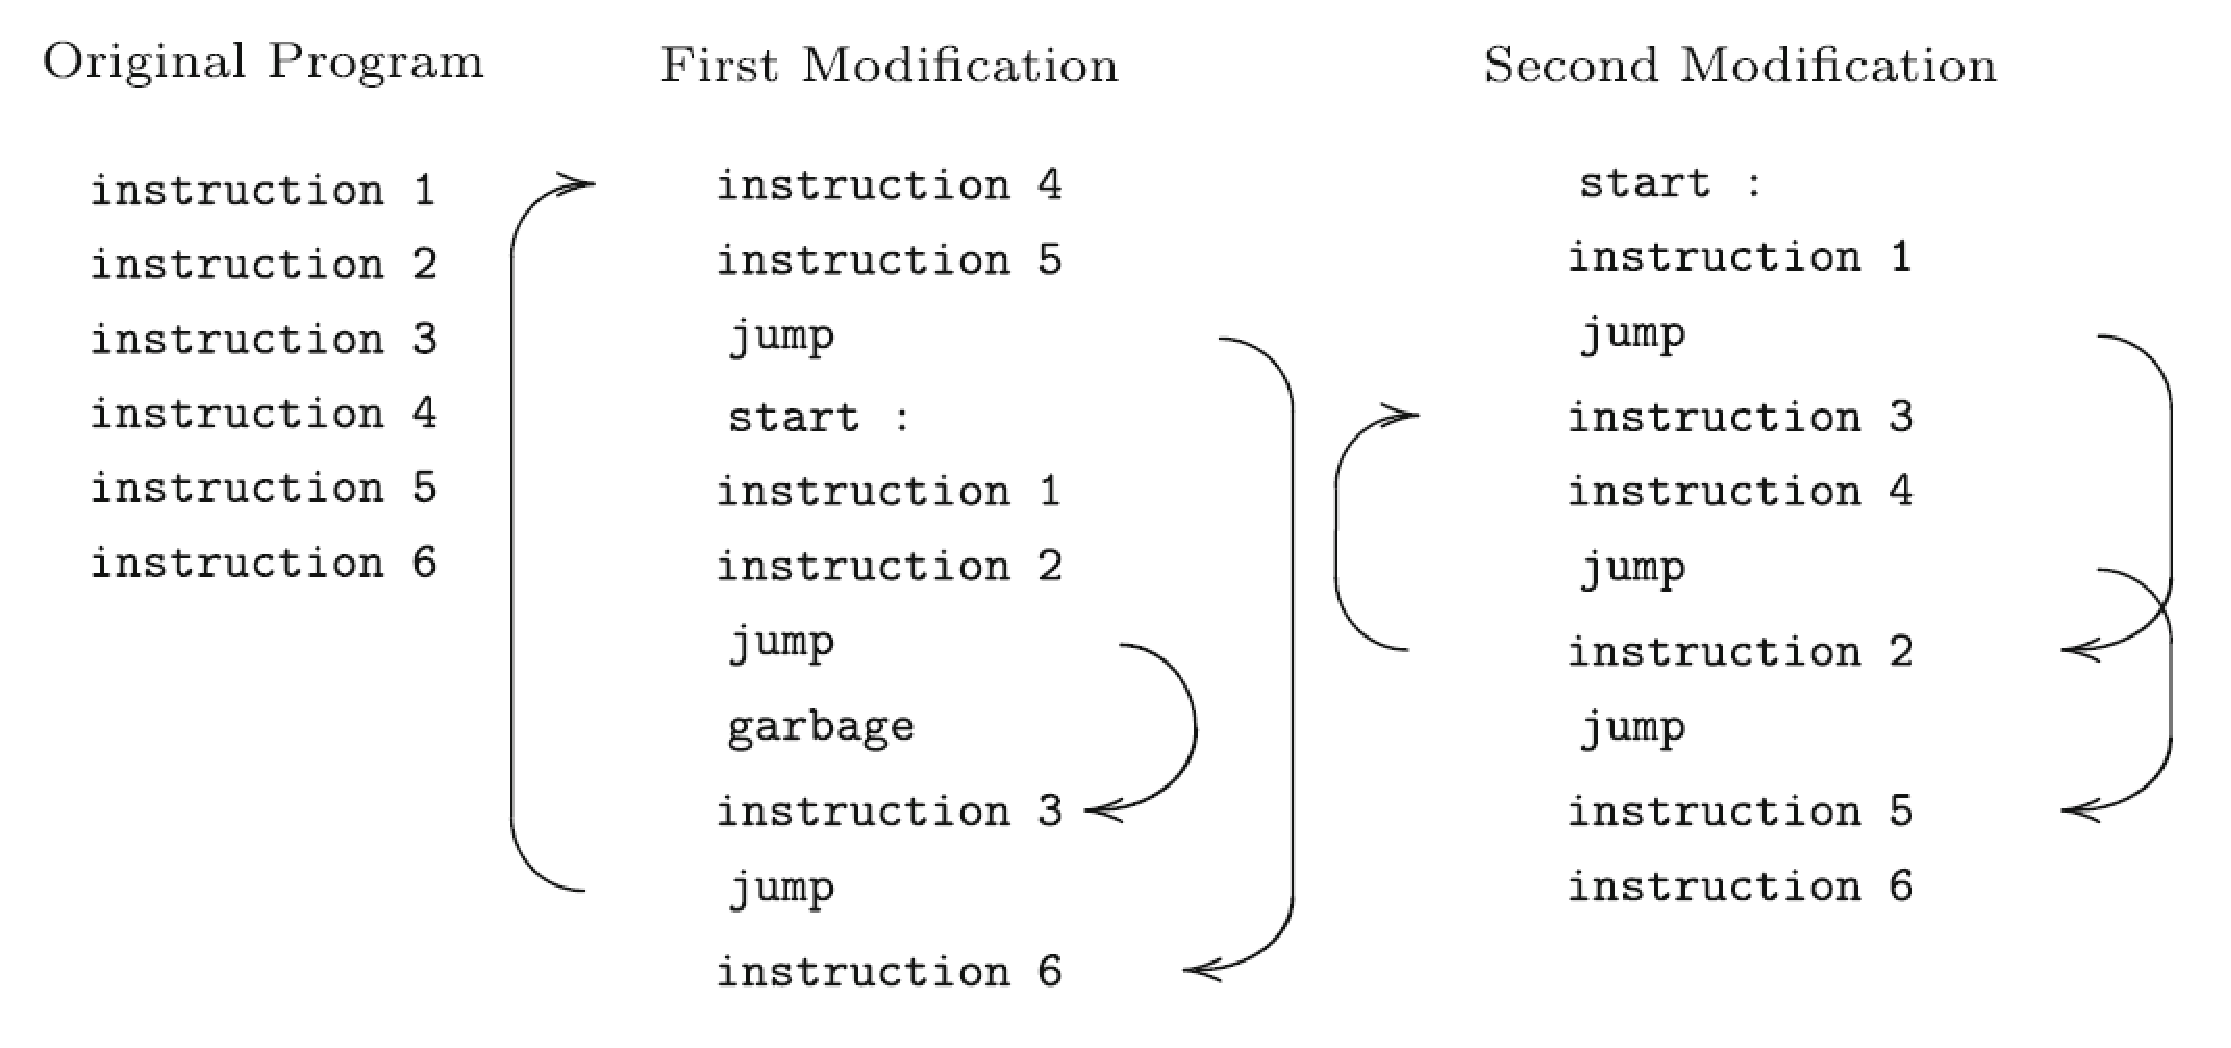
\includegraphics[scale=0.25]{input/GrapheJean1.eps}
\end{center}
\caption{Illustration de l'alt�ration du Control flow}
\end{figure}

\subsubsection*{Jump Table}

\noind Le but principal de l'utilisation des sauts est de faire en sorte que le d�sassembleur ne sache pas suivre le chemin d'un saut. Pour cela, on utilise tr�s g�n�ralement des sauts conditionnels dont la r�alisation d�pend de l'�tat d'un flag lors de l'ex�cution. On divise ainsi le programme en une succession de blocs d'instructions se terminant tous par un saut conditionnel. On construit alors une Jump Table qui d�termine l'�tat des variables bool�ennes qui d�finissent quels sauts doivent �tre suivis lors de l'ex�cution de mani�re � conserver le m�me enchainement des instructions bien qu'un saut inconditionnel soit fait � la fin de chaque bloc.\\

\noind Imaginons que l'on s�pare le programme en \textit{k} blocs. On construit alors \textit{k} variables bool�ennes Si tel que pour tout \textit{i} , si $K_{i}=\mathtt{True}$, alors le saut � la fin du \textit{i}�me bloc d'instructions est emprunt�. Si $K_{i}=\mathtt{False}$ on prend la branche par d�faut qui va envoyer le d�sassembleur vers un bloc qui n'est pas celui emprunt� normalement. \\

\noindent De la m�me mani�re, on peut utiliser les propri�t�s d'une suite pour calculer les valeurs prises par le flag. On peut imaginer que $K_{n}$ est la suite de syracuse ($K_{n+1}= K_{n/2}$ si paire et $3K_{n}+1$ sinon). Et incr�menter dans chaque bloc la suite et utiliser la conjecture (qu'au bout d'un certain rang \textit{n}, pour $K_{0}$ choisi on ait le cycle 4,2,1) afin de faire les tests appropri�s � la fin de chaque bloc pour que le saut choisi soit le bon. Si lors du d�sassemblage on ne trouve pas le bon $K_{0}$ pour lequel les $K_{n}$ vont prendre les valeurs attendues, l'ordre de d�sassemblage va �tre compl�tement faux\footnote{Ces suites sont ce qu'on appelle des clefs de d�sassemblage.}.\\

\noind Ces m�thodes ont pour but de rendre le plus obscure possible la destination des sauts de chaque bloc pour une personne qui cherche � d�sassembler. Cependant l'�volution de \textit{K} est bien connue de son cr�ateur et va d�terminer l'unique chemin valide que le programme doit suivre pour fonctionner.\\

\begin{figure}[hbtp]
\begin{center}
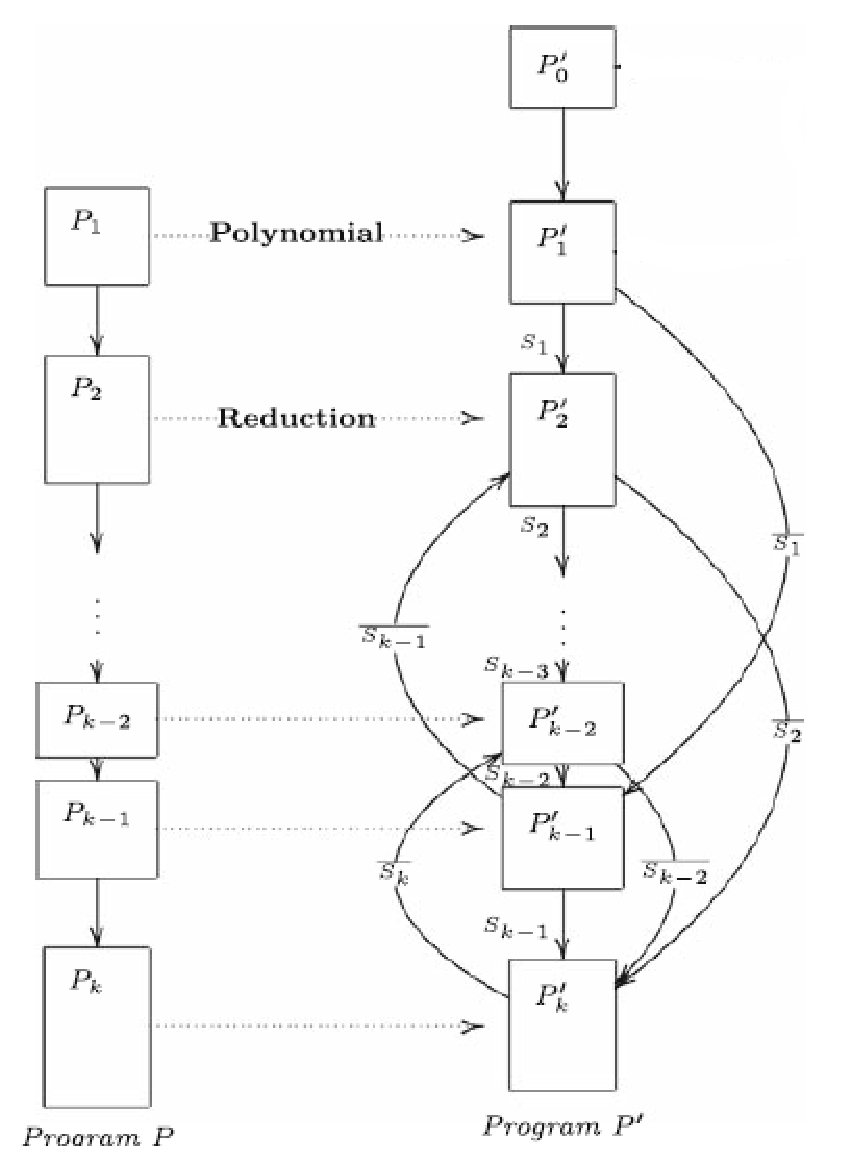
\includegraphics[scale=0.5]{input/GrapheJean2.eps}
\end{center}
\caption{Exemple d'obfuscation � l'aide d'une Jump Table}
\end{figure}
\subsubsection*{Opaque predicates}

\noind Le but consiste ensuite � rendre aussi incompr�hensible que possible le tableau de variables. On utilise alors des Opaque predicates qui permettent de faire en sorte qu'une variable bool�enne soit tout le temps vraie ou fausse tout en s'effor�ant de rendre aussi difficile que possible la connaissance de son �tat par un programme de d�sassemblage.

\noind Exemple : On sait que pour que l'ex�cution se passe correctement, il faut que la variable Sk soit vraie. On peut alors utiliser les instructions suivantes.

\begin{center}
\texttt{If(a*(a+1)\%2 == 0){ $S_{k}$ = true}
Else{ $S_{k}$ = false}}
\end{center}

\noindent O� \texttt{a} repr�sente un entier. Il est alors clair que la condition \texttt{a*(a+1)\%2 == 0} est toujours vraie cependant il est difficile pour un algorithme de d�sassemblage statique de d�terminer l'�tat de cette condition.

\subsubsection{Diff�rences entre data flow Obfuscation et control flow
Obfuscation}

\subsubsection*{Niveau d'abstraction}
\noind La diff�rence majeure entre ces deux classes de m�thodes d'obfuscation est qu'elles ne jouent pas sur le m�me niveau d'abstraction d'un programme. En effet, on pourrait dire que les m�thodes de modification de donn�es sont des m�thodes superficielles qui ne modifient pas l'essence du programme alors que les m�thodes de flow control sont des m�thodes qui modifient directement le graphe de flow d'un programme.
\subsubsection*{Diff�rents impacts sur les m�thodes de d�sassemblage}

\noind Nous avons vu en premi�re partie qu'il existait globalement 2 m�thodes de d�sassemblage : la m�thode Linear Sweep qui permet de suivre la progression du code de mani�re lin�aire sans prendre en compte les sauts et la m�thode Recursive Transerval qui permet de suivre les branches du graphe de flow et de d�sassembler le programme dans son ensemble en prenant en compte les sauts.

\noind Ainsi la m�thode d'insertion de junk instructions est utile pour contrecarrer la m�thode de d�sassamblage Linear Sweep. Les m�thodes de changement du flow control sont quant � elles utiles pour contrecarrer le d�sassemblage Recursive Traversal car son but est d'emp�cher les d�sassembleurs de pouvoir suivre les diff�rents sauts.

\subsection{Exemple d'obfuscateur}

\noind Dans cette partie nous allons pr�senter un exemple d'obfuscateur r�alis� par l'universit� d'Arizona et nous baser sur leurs r�sultats exp�rimentaux pour montrer l'efficacit� des m�thodes d'obfuscations.

\subsubsection{Pr�sentation de l'obfuscateur utilis�}

\noind La m�thode d'obfuscation utilis�e est la suivante : On divise le programme en un certain nombre de blocs. On fait terminer chacun de ces blocs par un saut conditionnel dont la condition est toujours soit vraie soit fausse de mani�re � conserver l'ordre d'ex�cution des instructions initial (Utilisation d'opaque predicates). 

\noind On remplace ensuite les sauts conditionnels suivant les blocs qui sont ex�cut�s un grand nombre de fois par des appels de fonctions (call en assembleur) ce qui permet une ex�cution plus rapide du programme. La distinction entre les blocs souvent ex�cut�s (qu'on appelle "hot") et les autres est effectu�e � l'aide d'un param�tre $\theta$ qui d�finit le pourcentage des blocs du programme qui seront consid�r�s comme ex�cut�s un grand nombre de fois.

\noind On effectue ensuite la comparaison entre le code assembleur obtenu par le d�sassemblage et le code assembleur qui correspond au programme initial (sans obfuscations) afin d'obtenir un facteur de confusion (pourcentage des instructions mal traduites).

\subsubsection{Pr�sentation des r�sultats}

\subsubsection*{Temps d'ex�cution}

\noind La premi�re constatation qui peut �tre faite est que le programme obfusqu� a un temps d'ex�cution plus grand que le programme initial. Cette diff�rence de temps d'ex�cution d�pend du param�tre $\theta$. En effet, $\theta$ grandit avec le nombre d'instruction "hot" et donc plus il y a d'appels de fonctions et donc plus le temps d'ex�cution est faible. Cela est du au fait qu'un \texttt{call} est plus rapide � ex�cuter qu'un \texttt{jne} en assembleur.

\noind Le tableau suivant repr�sente le quotient T1/T0, T1 �tant le temps d'ex�cution du programme obfusqu� et T0 celui du programme original. Les tests ont �t� r�alis�s sur plusieurs programmes et avec des param�tres $\theta$ diff�rents.

\begin{figure}[hbtp]

\begin{center}

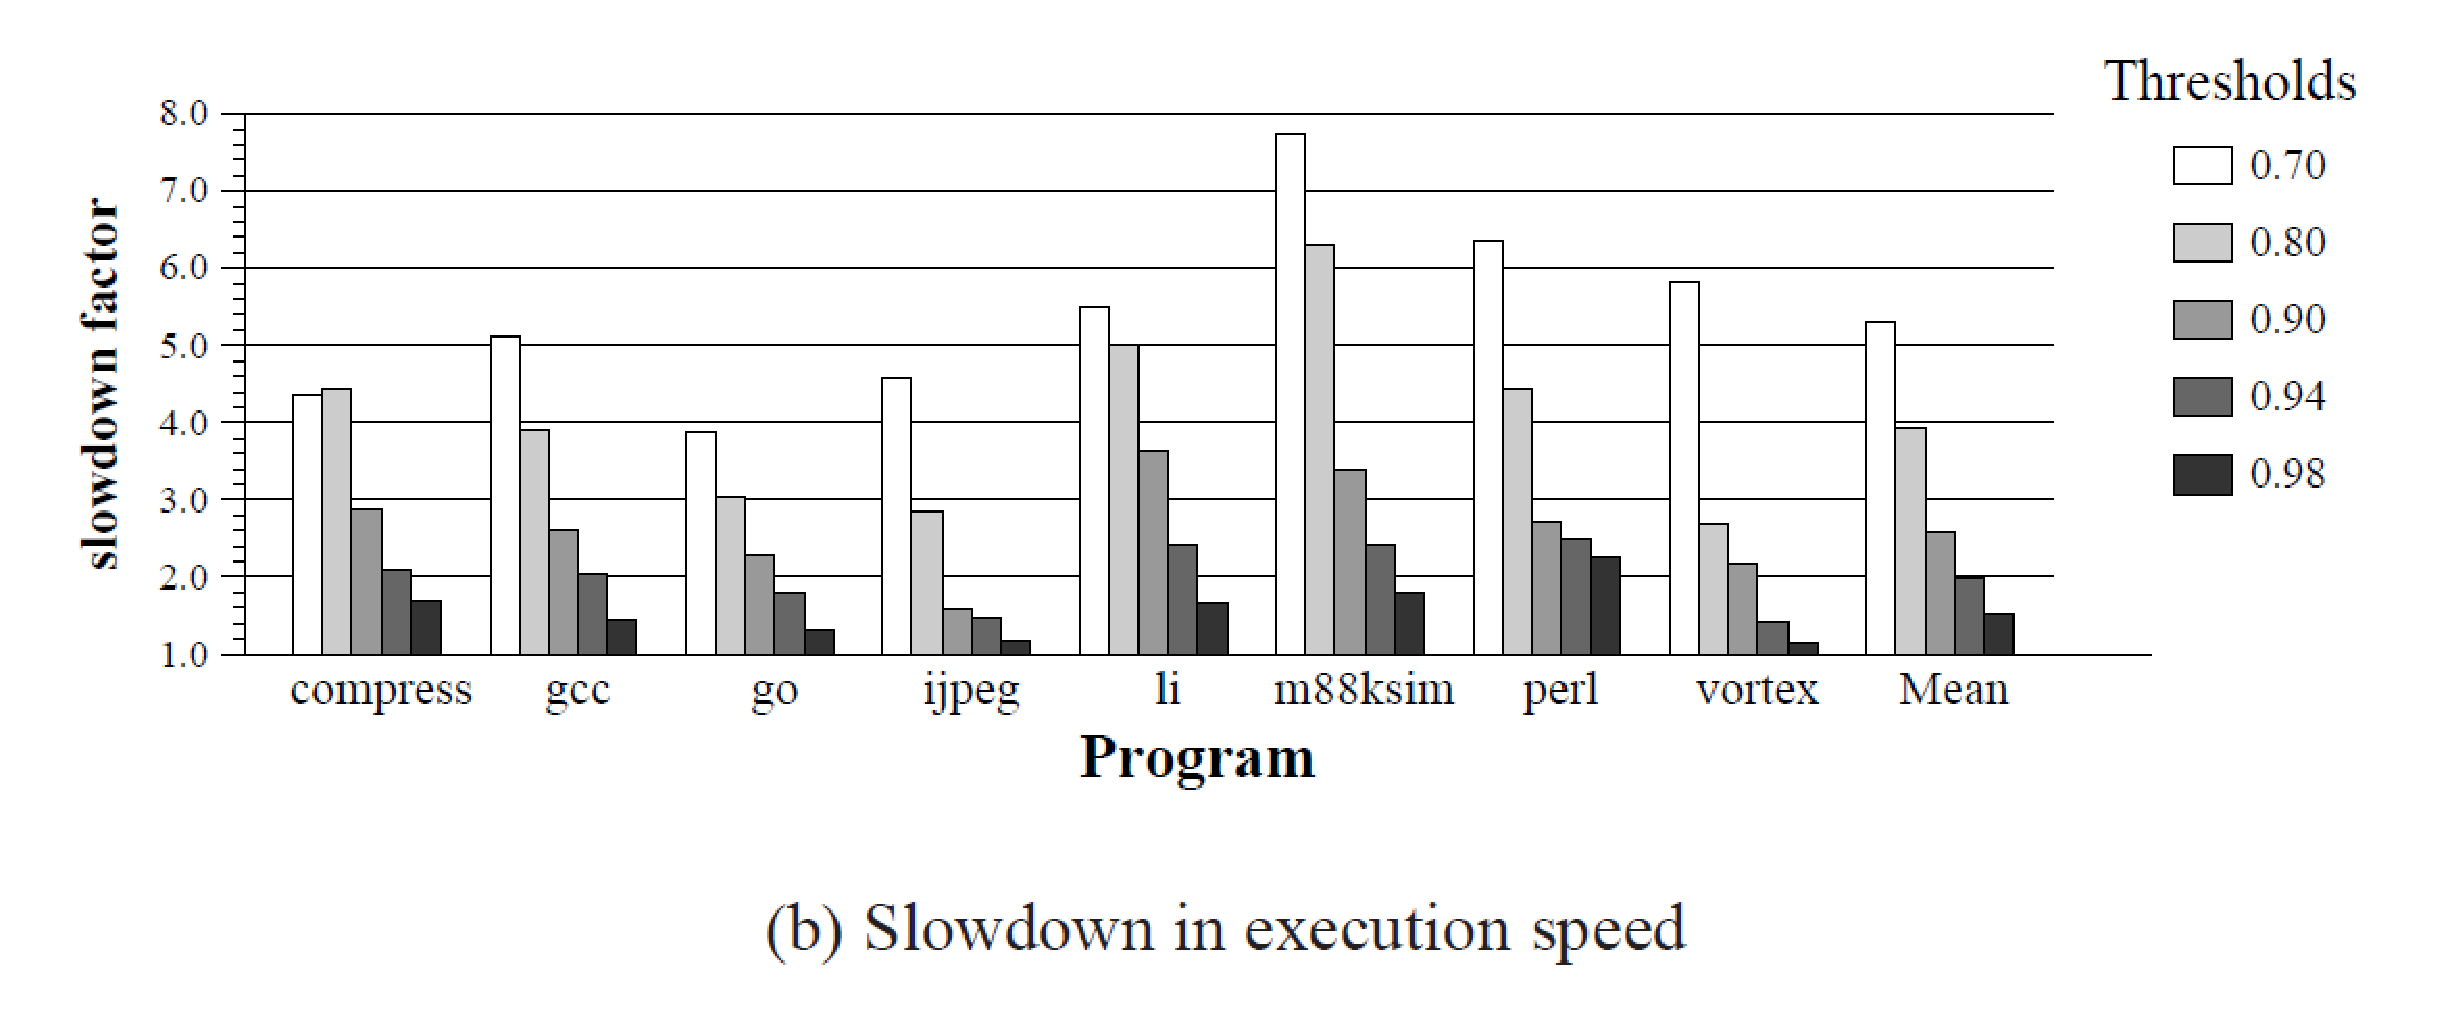
\includegraphics[scale=0.4]{input/GrapheJean3.eps}

\end{center}

\caption{Ralentissement apr�s obfuscation selon les compilateurs}

\end{figure} 

\subsubsection*{Taux d'erreur} 

\noind Le deuxi�me param�tre qu'il est important d'observer est le taux d'erreur du d�sassemblage. On distingue le taux d'erreur sur les blocs, le taux d'erreur sur les fonctions et le taux d'erreur sur les instructions. La diff�rence entre ces taux d'erreur est la suivante : On consid�re qu'un bloc ou une fonction est mal d�sassembl� si seulement une de ses instructions est mal d�sassembl�e. Le taux de confusion est ensuite donn� comme le pourcentage d'�l�ment mal d�sassembl�. Les tests sont effectu�s en utilisant les 2 m�thodes de d�sassemblage c'est � dire la m�thode r�cursive et la m�thode lin�aire.

\begin{figure}[hbtp]
\begin{center}
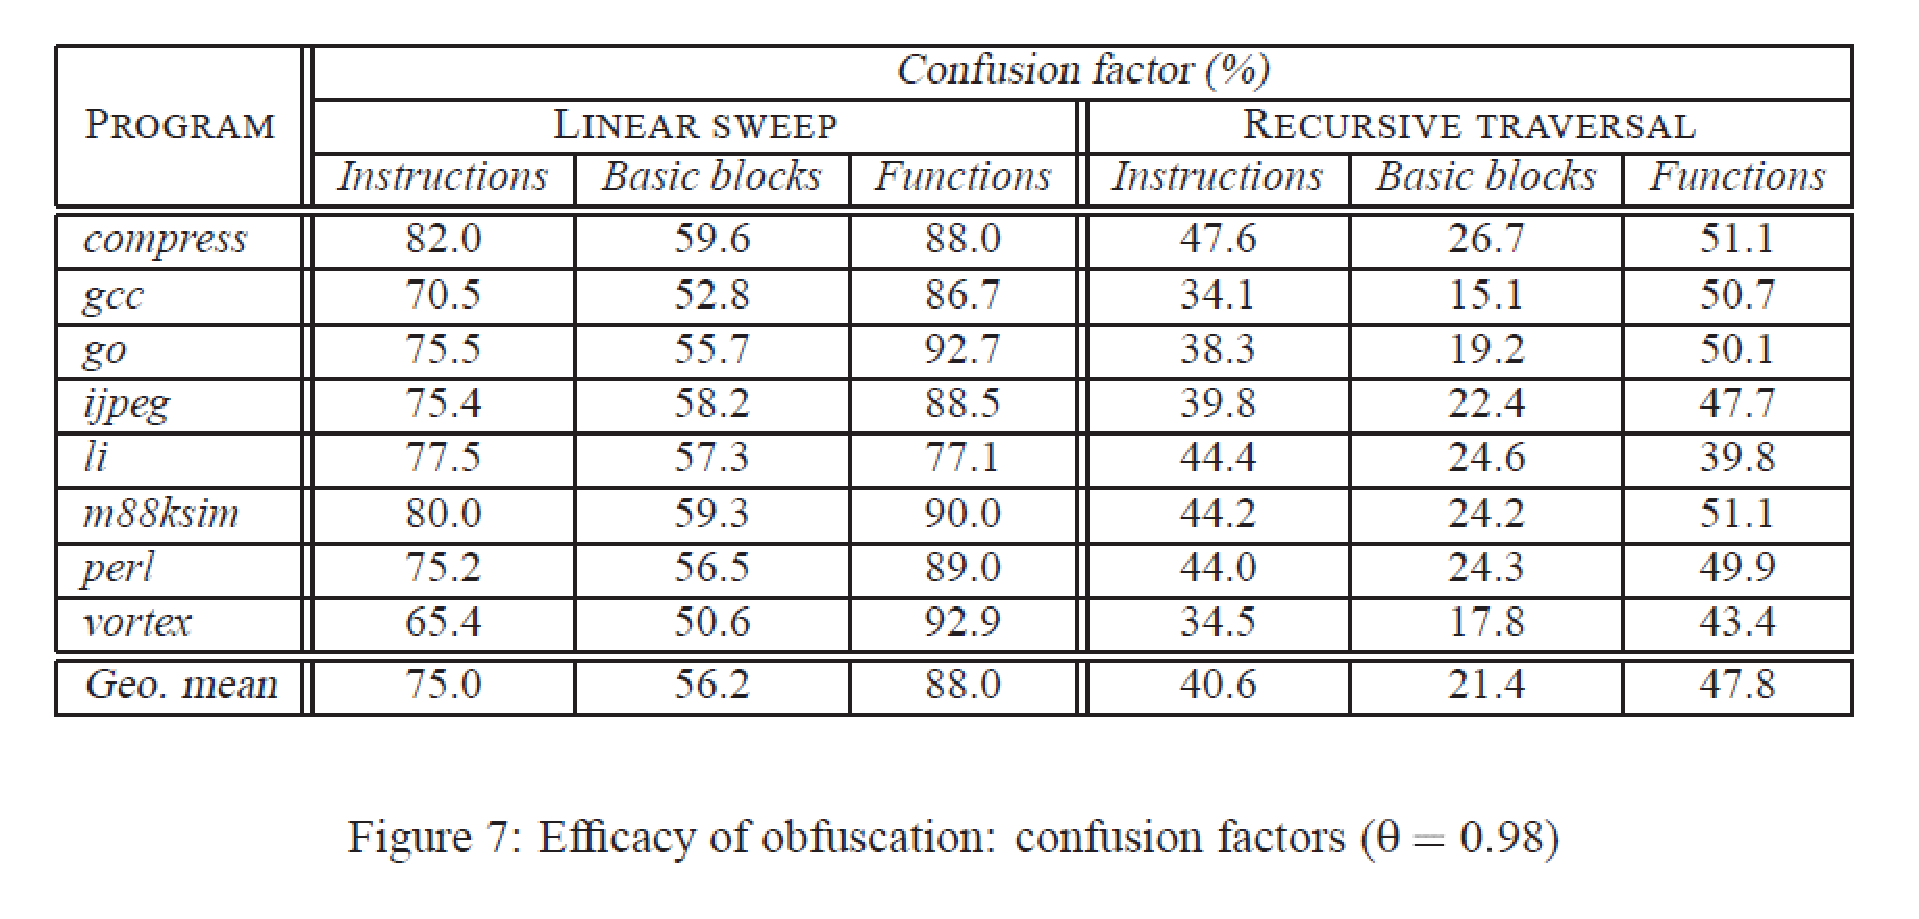
\includegraphics[scale=0.5]{input/GrapheJean4.eps}
\end{center}
\end{figure} 

\noind La premi�re constatation importante � faire est que le pourcentage d'erreur reste tr�s �lev� dans les 2 cas. On peut ensuite faire la constatation que la m�thode de d�sassemblage r�cursive est plus efficace et cela est du au fait comme nous l'avons d�j� vu que cette m�thode est bien plus robuste aux obfuscations qui jouent sur le graphe de Flow.



\section{Conventions du d�sassemblage}
	% !TEX root = ../main_final.tex

\noind Nous allons pr�senter ici comment s'effectue l'acquisition des donn�es, et comment les informations sont extraites du fichier ex�cutable.

\subsection{Construction du graphe de flow}

\noind Un d�sassemblage est d�fini par 3 param�tres : 

\begin{itemize}
\item L'adresse m�moire du point d'entr�e de l'ex�cutable charg� en m�moire
\item L'adresse virtuelle de ce point d'entr�e (c'est � dire l'adresse affich�e par le d�sassembleur)
\item La taille du bloc � d�sassembler.\\
\end{itemize}

\noind Apr�s lecture de ces donn�es (cf annexes), le d�sassembleur lit les instructions � partir de la premi�re et suit toutes les branches de mani�re r�cursive. Ainsi seules les branches atteignables par le programme sont d�sassembl�es\footnote{On verra par la suite que cette m�thode nous permettra de d�tecter les �tats inaccessibles, et surtout les \textit{junk bytes}, qui sont des instructions dont le d�but commence au milieu d'une autre.}. Le graphe de flow peut alors �tre extrait.

\noind Il est int�ressant de noter que lors du d�sassemblage on essaie autant que possible 
d'�viter les erreurs : en effet, toutes les instructions ne sont pas compr�hensibles � premi�re lecture. Par exemple, un \texttt{jmp rax} ne peut �tre compris � ce stade de l'�tude car on ignore la valeur contenue dans le registre \texttt{rax}. Afin de d�sassembler le maximum d'instructions possible, tout en s'arrangeant pour que le d�sassemblage garde un sens, nous avons adopt� des conventions d'arr�t ou de passage. Cependant, toutes les erreurs sont retenues dans le graphe. Dans de telles conditions, le d�sassemblage global ne stoppe jamais, mais l'�tude d'une branche s'arr�te pr�matur�ment si l'instruction suivante est ind�termin�e. L'ensemble des types d'erreurs est enregistr� dans une �num�ration (voir le listing \ref{erreurs}) d�crivant l'�tat de chaque n\oe ud du graphe\footnote{Elle contient �galement deux autres constantes permettant d'annoncer qu'un n\oe ud a plusieurs fils ou pas}.

\begin{lstlisting}[caption=�tats possibles d'un n\oe ud, label=erreurs, float=htb]
enum ValeurEtat{
    SANS_INTERET,
    GO_AND_LEAVE,
    OPCODE_INCONNU,
    DEPASSEMENT_BLOC,    
    SAUT_INCOND_OUT_OF_BLOCK,
    SAUT_INCOND_INDEFINI,
    FIN_BLOC_SANS_POINT_ARRET,
    CALL_TERMINAL_OOB,
    CALL_TERMINAL_INDEFINI,
    CALL_FIN_BLOC,
    CALL_INDEFINI,
    CALL_OUT_OF_BLOCK,
    SAUT_COND_FIN_BLOC,
    SAUT_COND_INDEFINI,
    SAUT_COND_OUT_OF_BLOCK,
    SAUT_COND_TERMINAL,
};
\end{lstlisting}

\paragraph{Les sauts hors du bloc} sont souvent dus � des appels de fonctions dynamiquement li�es. Ces cas de passage sont reper�s par les constantes 
\begin{itemize}
\item\texttt{CALL\_OUT\_OF\_BLOCK},
\item \texttt{CALL\_TERMINAL\_OOB},
\item \texttt{SAUT\_INCOND\_OUT\_OF\_BLOCK},
\item \texttt{SAUT\_COND\_OUT\_OF\_BLOCK}.
\end{itemize}

\paragraph{Les erreurs de lecture} sont dues � un probl�me lors du d�sassemblage d'une instruction. Elles peuvent �tre provoqu�es par la lecture d'un opcode inconnu (\texttt{OPCODE\_INCONNU}) ou d'un d�passement du bloc lors de la lecture de cette instruction(\texttt{DEPASSEMENT\_BLOC}).

\paragraph{Les sauts ind�finis} sont provoqu�s par l'utilisation de la valeur d'un registre ou d'un emplacement m�moire comme adresse de saut (par exemple \texttt{jmp rax}). Ils sont rep�r�s par les constantes
\begin{itemize}
\item \texttt{SAUT\_INCOND\_INDEFINI},
\item \texttt{SAUT\_COND\_INDEFINI},
\item \texttt{CALL\_INDEFINI}, 
\item \texttt{CALL\_TERMINAL\_INDEFINI}.
\end{itemize}

\paragraph{Les op�rations en fin de blocs} diff�rentes d'un \texttt{ret}, d'un \texttt{jmp} ou d'un \texttt{hlt} l�vent une erreur car il existe une branche dont le chemin est ind�termin�. Les constantes utilis�es pour ce type d'erreur sont 
\begin{itemize}
\item \texttt{CALL\_TERMINAL\_OOB},
\item \texttt{CALL\_TERMINAL\_INDEFINI},
\item \texttt{CALL\_FIN\_BLOC},
\item \texttt{SAUT\_COND\_FIN\_BLOC}.
\end{itemize}

\subsection{M�thode de repr�sentation}

\subsubsection{Dans le programme}

\noind Lors du chargement du programme en m�moire, � chaque octet est associ� un n\oe ud. D'autre part, chaque instruction est repr�sent�e par le n\oe ud associ� � son premier octet. Les autres n\oe uds sont alors marqu�s comme recouverts\footnote{Pour �conomiser de la place, chacun de ses n\oe uds pointe vers le m�me n\oe ud}. Puis, lors du d�sassemblage en suivant les branchements, ces n\oe uds sont reli�s entre eux pour former le graphe.

\subsubsection{Repr�sentation persistante}

\noind Nous utilisons la structure des fichiers \texttt{.dot} coupl� au logiciel \texttt{graphviz} pour avoir une repr�sentation graphique de graphe que nous avons construit. On s'interresse ici � la structure du graphe et pas � une �tude qualitative de chaque n\oe ud. C'est pourquoi le graphe obtenu dans l'�tape de construction est trait� au pr�alable par une fonction de simplification qui supprime les n\oe uds ayant un unique fils et �tant lui-m�me fils d'un n\oe ud � fils unique. 

\noind La figure \ref{CFGfibo} page \pageref{CFGfibo} donne le graphe de flow pour le programme \texttt{fibo} (listing \ref{fiboasm}) : Les n\oe uds rouges repr�sentent les \texttt{call}, les bleus les \texttt{jmp}, les verts les sauts conditionnels et les gris les \texttt{ret} et \texttt{hlt}. Les fl�ches rouges d�signent la nouvelle fonction appel�e et les vertes le chemin si le saut est valide.

\noind La construction du graphe de flow est une premi�re �tape dans le travail de  d�sassemblage au sens large. L'�tude va porter � pr�sent sur la s�mantique des instructions en s'appuyant sur ce graphe. Le but sera de mettre en �vidence le maximum d'informations possible, soit en simplifiant le graphe, soit en l'�tendant aux branches ind�finies en d�terminant les sauts.

\subsubsection{Application : d�tection des \jbs}

\noind Un \jb est le recouvrement d'une instruction par une autre : une instruction s'�crit en g�n�ral sur plus d'un octet. Si tel est le cas, un saut permet tr�s facilement de placer le registre IP entre deux instructions, adresse normalement inaccessible en cas de lecture lin�aire. La figure \ref{junk} donne une illustration d'une telle manipulation.

\begin{figure}[htb]
\centering 
\includegraphics[width=9cm]{input/junk.eps}
\caption{Principe du \textit{junk byte}}
\label{junk}
\end{figure}

\noind La d�tection des \jbs est permise par la repr�sentation de chaque instruction par le n\oe ud associ� � son premier octet et par le marquage des n\oe uds suivants comme "recouverts". En effet, s'il existe un n\oe ud du graphe qui poss�de la qualit� d'�tre recouvert, ce n\oe ud est par cons�quent issue d'un \jb\!. Cette m�thode nous permet de localiser tous les \jbs issus de la premi�re passe de d�sassemblage.

\begin{center}
\begin{pspicture}(0,-2.4715624)(10.22,2.4715624)
\definecolor{color693b}{rgb}{0.9333333333333333,0.06666666666666667,0.06666666666666667}
\psframe[linewidth=0.004,dimen=outer,fillstyle=solid,fillcolor=color693b](8.0,-0.226875)(4.4,-0.426875)
\psframe[linewidth=0.004,dimen=outer,fillstyle=solid,fillcolor=color693b](3.8,-0.226875)(1.4,-0.426875)
\psline[linewidth=0.04cm,arrowsize=0.05291667cm 2.0,arrowlength=1.4,arrowinset=0.4]{->}(0.6,-0.426875)(10.2,-0.426875)
\psline[linewidth=0.04cm,linestyle=dashed,dash=0.16cm 0.16cm](0.0,-0.426875)(0.6,-0.426875)
\psline[linewidth=0.04cm,linestyle=dotted,dotsep=0.16cm](0.2,-0.426875)(0.0,-0.426875)
\psline[linewidth=0.04cm,linestyle=dotted,dotsep=0.16cm](0.2,-0.426875)(0.0,-0.426875)
\psline[linewidth=0.04cm](0.8,-0.426875)(0.8,-0.226875)
\psline[linewidth=0.04cm](1.4,-0.226875)(1.4,-0.426875)
\psline[linewidth=0.04cm](2.0,-0.226875)(2.0,-0.426875)
\psline[linewidth=0.04cm](2.6,-0.226875)(2.6,-0.426875)
\psline[linewidth=0.04cm](3.2,-0.226875)(3.2,-0.426875)
\psline[linewidth=0.04cm](3.8,-0.226875)(3.8,-0.426875)
\psline[linewidth=0.04cm](4.4,-0.226875)(4.4,-0.426875)
\psline[linewidth=0.04cm](5.0,-0.226875)(5.0,-0.426875)
\psline[linewidth=0.04cm](5.6,-0.226875)(5.6,-0.426875)
\psline[linewidth=0.04cm](6.2,-0.226875)(6.2,-0.426875)
\psline[linewidth=0.04cm](6.8,-0.226875)(6.8,-0.426875)
\psline[linewidth=0.04cm](7.4,-0.226875)(7.4,-0.426875)
\psline[linewidth=0.04cm](8.0,-0.226875)(8.0,-0.426875)
\psline[linewidth=0.04cm](8.6,-0.226875)(8.6,-0.426875)
\psline[linewidth=0.04cm](9.2,-0.226875)(9.2,-0.426875)
\psbezier[linewidth=0.04](0.8,-0.626875)(0.8,-1.426875)(3.8,-1.426875)(3.8,-0.626875)
\psline[linewidth=0.04cm,arrowsize=0.05291667cm 2.0,arrowlength=1.4,arrowinset=0.4]{->}(2.2,-1.226875)(2.2,-1.826875)
\usefont{T1}{ppl}{m}{n}
\rput(2.0035937,-2.326875){\small Add eax ebx}
\psline[linewidth=0.04cm,arrowsize=0.05291667cm 2.0,arrowlength=1.4,arrowinset=0.4]{->}(1.0,1.973125)(1.0,-0.226875)
\usefont{T1}{ppl}{m}{n}
\rput(2.3978126,2.273125){\small premier octet de l'instruction}
\psline[linewidth=0.04cm,arrowsize=0.05291667cm 2.0,arrowlength=1.4,arrowinset=0.4]{->}(3.0,1.173125)(1.6,-0.226875)
\psline[linewidth=0.04cm,arrowsize=0.05291667cm 2.0,arrowlength=1.4,arrowinset=0.4]{->}(3.0,1.173125)(2.4,-0.226875)
\psline[linewidth=0.04cm,arrowsize=0.05291667cm 2.0,arrowlength=1.4,arrowinset=0.4]{->}(3.0,1.173125)(3.0,-0.226875)
\psline[linewidth=0.04cm,arrowsize=0.05291667cm 2.0,arrowlength=1.4,arrowinset=0.4]{->}(3.0,1.173125)(3.6,-0.226875)
\usefont{T1}{ppl}{m}{n}
\rput(5.500781,1.473125){\small Octets marqu�s comme recouverts}
\psbezier[linewidth=0.04](3.8,-0.626875)(3.8,-1.426875)(8.0,-1.426875)(8.0,-0.626875)
\psline[linewidth=0.04cm,arrowsize=0.05291667cm 2.0,arrowlength=1.4,arrowinset=0.4]{->}(6.0,-1.226875)(6.0,-1.826875)
\usefont{T1}{ppl}{m}{n}
\rput(5.894375,-2.326875){\small Mov ebx 0x7830432}
\psline[linewidth=0.04cm,arrowsize=0.05291667cm 2.0,arrowlength=1.4,arrowinset=0.4]{->}(6.2,1.173125)(4.8,-0.226875)
\psline[linewidth=0.04cm,arrowsize=0.05291667cm 2.0,arrowlength=1.4,arrowinset=0.4]{->}(6.2,1.173125)(5.4,-0.226875)
\psline[linewidth=0.04cm,arrowsize=0.05291667cm 2.0,arrowlength=1.4,arrowinset=0.4]{->}(6.2,1.173125)(5.8,-0.226875)
\psline[linewidth=0.04cm,arrowsize=0.05291667cm 2.0,arrowlength=1.4,arrowinset=0.4]{->}(6.2,1.173125)(6.6,-0.226875)
\psline[linewidth=0.04cm,arrowsize=0.05291667cm 2.0,arrowlength=1.4,arrowinset=0.4]{->}(6.2,1.173125)(7.2,-0.226875)
\psline[linewidth=0.04cm,arrowsize=0.05291667cm 2.0,arrowlength=1.4,arrowinset=0.4]{->}(6.2,1.173125)(7.8,-0.226875)
\end{pspicture}
\end{center}

\subsection{Propagation des constantes}

\noind Cette m�thode a pour but d'expliciter les constantes pour chaque \noeud du graphe. Ayant une meilleure connaissance de ces constantes, l'interpr�tation du graphe sera plus facile.

\subsubsection{Adaptation de la m�thode}

\noind L'\algo donn� par \textsc{Kildall} \cite{kildall} utilise une structure de liste afin de comptabiliser l'ensemble des \noeuds dont les constantes doivent �tre mises � jour. Nous avons pr�f�r� utiliser le programme r�cursif suivant en pseudo-code

\begin{lstlisting}[caption=propagation des variables, label=prop,numbers=left, numberstyle=\tiny]
static void optimizePool_aux(Noeud* n, Noeud* pere){
	Pool* copyPool = newPoolCopy(pere->pool);
	f(pere, copyPool);
	// f modifie copyPool et y stock le nouveau pool
	int inc = incluDans(n->pool, copyPool);
	if (inc != NON_INCLUS){
		delete(copyPool);
		return;
	}
	inter(n->pool, copyPool); // intercection dans n->pool
	delete(copyPool);
	List* list = n->listeFils;
	if (list == NULL) {
		return;
	}
	for (Noeud* N in list) {
		optimizePool_aux(N, n);
	}
}
void optimizePool(Noeud* n, const Processeur* initialPool){
	int inc = incluDans(g->pool, initialPool);
	if (inc != NON_INCLUS){
		return;
	}
	inter(n->pool, initialPool); // intercection dans n->pool
	if (n->listeFils == NULL) {
		return;
	}
	List* list = n->listeFils;
	for (Noeud* N in list) {
		optimizePool_aux(N, n);
	}
}
\end{lstlisting}

\noind Il est relativement simple de constater que cet algorithme est �quivalent � celui donn� pr�c�demment, except� l'appel r�cursif des lignes 17 et 31. En effet, cet appel pouvant modifier le pool $n$, l'ensemble des appels sur les fils de $n$ n'est pas consistant. Cependant, on d�montrera en annexe (page \pageref{demo_pc_rec}) que le r�sultat est inchang�. 

\noind Cette impl�mentation a plusieurs avantages dont celui d'optimiser l'utilisation m�moire. En effet, chaque pool peut prendre beaucoup de place en m�moire (de l'ordre du Ko pour un seul \noeud\!). Alors que l'\algo initial demande la cr�ation d'un nouveau pool pour chaque appel r�cursif, notre \algo se d�roule en taille m�moire constante.

\subsubsection{All�gement du graphe}

\noind L'\algo de propagation des constantes permet de conna�tre l'�tat des registres � chaque \noeud\!, en particulier pour le registre de flags. Ce registre d�terminant le d�roulement du programme, la connaissance d'un drapeau pourra �ventuellement permettre de supprimer des branches du graphe original. Si tel est le cas, on appliquera une nouvelle fois l'algorithme de propagation des constantes pour tenir compte de ce "d�branchement".

\subsubsection{D�termination des sauts ind�finis} De m�me, il sera �ventuellement possible de cr�er de nouvelles branches si des sauts dont l'adresse cible est \textit{a priori} inconnue sont d�termin�s par la propagation des constantes. \textbf{Cependant}, il convient de remarquer que cette nouvelle branche peut diminuer la d�termination du graphe. En effet, si elle rejoint un \noeud du graphe d�j� existant, elle peut induire des modifications sur les variables d�terminis�es avant branchement.


%\subsection{�tude formelle des variables}


	
\section{Utilisation du d�sassembleur}
	% !TEX root = ../main_final.tex

\noind Nous avons essay� d'impl�menter le d�sassembleur d'une mani�re la plus modulaire possible.
Bien que notre d�sassembleur ne prenne en compte pour l'instant que peu d'instructions assembleur, nous avons fait en sorte
que l'impl�mentation future de nouvelles instructions soit simple. D'autre part nous avons essay� de rendre son utilisation assez souple (chargement d'un programme et analyse pour Mach-o et ELF automatique) et surtout transparente. C'est pour cela que le code est tr�s comment�.

\subsection{Organisation des fichiers sources}

\subsubsection{Contenu des fichiers}


\noind Chaque fichier \texttt{.c} autre que \texttt{main.c} et \texttt{test.c} est accompagn� d'un fichier header donnant le prototype des fonctions r�utilisables dans les autres fichiers. Il y a �galement quelques fichiers header suppl�mentaires comprenant 
\begin{itemize}
\item l'ensemble des constantes du programme (\texttt{macro.h})
\item des macros permettant d'acc�der � la saisie de code uniquement (et donc \textit{a priori} inutile apr�s compilation de la biblioth�que) (dans le fichier \texttt{\_macro\_Build.h}). Ces macros permettent entre autres d'acc�der facilement au registre d'un processeur simplement en invoquant son nom (par exemple invoquer le registre eax par \texttt{\_EAX}) pourvu que le processeur s'appelle \texttt{proc}.
\end{itemize}

\subsubsection{D�pendances}

\noind Le projet ne d�pend que des biblioth�ques \bea et \texttt{libelf} pour son utilisation. Les classes de test requi�rent en plus la biblioth�que C-unit.


\subsection{Machine virtuelle}

\noind Afin d'avoir le maximum d'informations sur les effets du programme sans pour autant l'ex�cuter, nous essayons de faire virtuellement toutes les op�rations faites par un programme sur un processeur simul�.

\subsubsection{Classe}

\noind En accord avec l'\algo de \textsc{Kildall}, chaque variable doit �tre associ�e � une classe. Dans le simple cas de la propagation des constantes, les deux classes sont \classedef et \classendef\!. C'est pourquoi chaque variable d�finie par la suite devra se rapporter � une classe.

\subsubsection{Registres}

\noind La difficult� pour les registres a �t� de pouvoir g�rer l'appel de n'importe quel sous-registre, tout en garantissant que la modification d'un registre d'une famille (par exemple la famille \texttt{RAX}, \texttt{EAX}, \texttt{AX}, \texttt{AH}, \texttt{AL}) modifie de mani�re ad�quate les autres registres de la famille. On voulait �galement que l'appel � un registre soit simple et puisse se faire directement. Pour cela, nous avons choisi (comme on peut le voir avec les registres filsl(ow) et filsh(igh) dans la structure) de repr�senter les registres par un arbre binaire. On peut donc adapter la taille des registres et le nombre et/ou la taille de ses subdivisions.

\begin{lstlisting}[caption=Structure de registre, label=prop]
typedef struct _registre{ // 32 bytes
    int                 taille;
    uint64_t            valeur; 
    int                 classe;
    struct _registre*   filsl;
    struct _registre*   filsh;
}Registre;
\end{lstlisting}

\noind Les fonctions principales permettant de g�rer les registres sont les suivantes :\\
\begin{itemize}
\item \texttt{uint64\_t getRegVal(const Registre* reg)} permet d'acc�der � la valeur d'un registre et ce quelle que soit la classe de ce registre.
\item \texttt{uint64\_t setRegVal(Registre* reg, uint64\_t n)} permet d'affecter une valeur � un registre. Si le registre ou l'un de ses fils est de classe \classendef, ce registre ou ce fils passe � la classe \classedef\!.
\item \texttt{int getRegClassRec(Registre*)} donne la valeur de la classe du registre ainsi que celle de fils. Ainsi, cette fonction renvoie \classendef \ssi le registre ou l'un de ses fils est de la classe \classendef\!.
\item \texttt{void setRegClassRec(Registre*, int classe)} affecte au registre et � l'ensemble de ses fils la classe \texttt{classe}.
\end{itemize}

\subsubsection{M�moire}

\noind Nos pr�occupations en ce qui concerne la gestion de la m�moire virtuelle ont �t� les m�mes que celles au sujet des registres : l'acc�s � n'importe quel segment m�moire devait �tre simple et devait tenir compte des cases m�moire et les changer correctement s'il le fallait. Pour cela, il a fallu mettre en place plusieurs structures, � commencer par la m�moire de la machine. Elle est cod�e en \C \! comme le montre le listing \ref{mem_def}.

\begin{lstlisting}[caption=Structure de la m�moire, label=mem_def]
typedef struct _byte{
    uint64_t virtualAddr;
    uint8_t val;
    uint8_t classe;
}Byte;

typedef  struct _memoire {
    uint64_t size;
    uint64_t sizeAllocatedMemory;
    Byte** tabBytes;
}Memoire;
\end{lstlisting}

\noind Une m�moire est un tableau de \texttt{Byte}s \imp{tri�s par adresse m�moire}, chacun connaissant cette adresse. Cette repr�sentation permet une gestion relativement ais�e de la m�moire, les acc�s se faisant par recherche dichotomique du \texttt{Byte} recherch�, et l'�criture �crivant sur chacun des \texttt{Byte}s concern�s, les cr�ant si n�cessaire.\\

\noind La seconde structure est l'�quivalent des registres pour la m�moire. Il s'agit des segments m�moire :

\begin{lstlisting}[caption=Segment m�moire]
typedef struct _segment{
    Memoire* mem;
    uint64_t virtualAddr;
    uint8_t taille; // en octet
}Segment;
\end{lstlisting}

\noind Les fonctions importantes pour la gestion m�moire sont les suivantes :\\

\begin{itemize}
\item \texttt{int* getSegClassRec(Segment seg)} donne la classe d'un segment m�moire. Si le segment comporte des \texttt{Byte}s non d�finis dans le tableau, la fonction renvoie l'entier \classendef\!.
\item \texttt{uint64\_t getSegVal(Segment seg)} donne la valeur du segment donn�. Cette fonction ne peut �tre utilis�e sur un segment de classe \classendef car les cases m�moires ne sont peut-�tre m�me pas d�finies dans le tableau.
\item \texttt{void setSegClassRec(Segment, int classe)} attribue � tous les \texttt{Byte}s du segment la classe \texttt{classe}. Si besoin la fonction cr�e les \texttt{Byte}s qui manquent.
\item \texttt{uint64\_t setSegVal(Segment seg, uint64\_t val)} assigne � tous les \texttt{Byte}s d'un segment la valeur donn�e et fait passer ces bytes � la classe \classedef si ils sont � la classe \classendef\!. De m�me, si besoin il y a, la fonction cr�e les \texttt{Byte}s manquants.
\end{itemize}

\subsubsection{Variable}

\noind Le type \texttt{Variable} est un \textit{wrapper} permettant de manipuler ind�pendamment les \texttt{Registre}s et les \texttt{Segment}s. Il est d�fini en \C de cette mani�re :

\begin{lstlisting}[caption=Structure d'une Variable]
typedef struct _variable{
    uint8_t type;
    Registre* reg;
    Segment seg;
}Variable;
\end{lstlisting}

\noind Les fonctions utiles sont elles m�mes pour la plupart des \textit{wrappers} des fonctions des \texttt{Registre}s et des \texttt{Variable}s : \\

\begin{itemize}
\item \texttt{uint64\_t getVarVal(Variable)}

\item \texttt{int getVarClassRec(Variable)}

\item \texttt{uint64\_t setVarVal(Variable, uint64\_t)}

\item \texttt{int getVarTaille(Variable)} donne la taille de la variable \imp{en bits}\!.

\item \texttt{void setVarClassRec(Variable, int classe)}
\end{itemize}

\subsubsection{Pile d'appel}

\noind Pour finir la simulation hardware, on a cr�� un mod�le de pile d'appel. Elle utilise la \texttt{Memoire} pour stocker les informations sous forme d'une liste cha�n�e de \texttt{Segment}s. Les fonctions essentielles sont :\\

\begin{itemize}
\item \texttt{void pushStack(Stack*, Variable, Registre* \_RSP)}
\item \texttt{void popStack(Stack*, Variable, Registre* \_RSP)}
\end{itemize}

\subsubsection{Processeur}

\noind Comme nous nous int�ressons aux changement d'�tat de l'ordinateur nous avons du simuler le processeur. Nous avons choisi de repr�senter le processeur par 3 attributs, la structure de pile, un tableau de registres de flag contenant 9 flags, et un tableau de registres contenant 80 registres. Ce choix de repr�sentation par tableau, permet de r�utiliser le programme avec des processeurs avec diff�rents flags, registres; donc diff�rents types de processeurs.


\begin{lstlisting}[caption=structure du processeur, label=prop]
typedef struct _Processeur{ // 664 bytes
    Stack* stack;
    Registre*   tabRegistre[NOMBRE_REGISTRES];
    uint8_t     tabFlags[NOMBRE_FLAGS]
}Processeur;
\end{lstlisting}

\noind Le diagramme de classe du hardware de la machine virtuelle est donn� dans la figure \ref{struct_proc}.

\begin{figure}[htb]
\centering
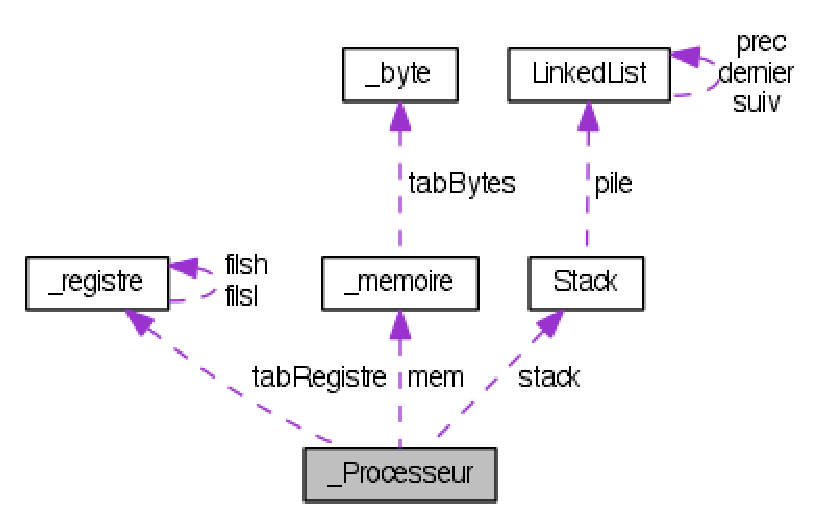
\includegraphics[width=7cm]{input/struct___processeur__coll__graph.eps}
\caption{Diagramme de classe du hardware de la machine virtuelle}
\label{struct_proc}
\end{figure}

\subsection{Impl�mentation des instructions}

\subsubsection{Mode de repr�sentation}

\noind Afin de pourvoir suivre l'�tat des registres, il faut connaitre l'effet des Instructions assembleur sur ces registres. Nous avons 
donc du cr�er une structure en m�moire qui permet de simuler l'action des instructions sur les diff�rents registres. 
Nous avons essay� de simuler le paradigme de la POO dans la cr�ation de nouvelles fonctions d'instructions afin que l'on puisse en rajouter facilement. 
Pour prendre en compte les actions d'une nouvelle instruction, il suffit de cr�er les fonctions qui vont modifier les registres de flags de la m�me mani�re que l'instruction va le faire.

\begin{lstlisting}[caption=structure d'instructions, label=prop,numbers=left, numberstyle=\tiny]
typedef struct _instruction{
    int(*of_aux)(const Registre*,const Registre*,const Registre*);
    int(*cf_aux)(const Registre*,const Registre*,const Registre*);
    int(*af_aux)(const Registre*,const Registre*,const Registre*);
    int zf_aux;         
    int pf_aux;         
    int sf_aux; 
    Registre* (*f)(Registre*,Registre*,Registre*,Processeur*,int);
}Instruction;
\end{lstlisting}

\subsubsection{Ajout d'une instruction}

\noind La cr�ation des instruction doit s'appuyer sur la documentation Intel\cite{intel}. L'exemple suivant, va illustrer la proc�dure � suivre pour rajouter au d�sassembleur une Instruction. \\

 
\begin{lstlisting}[caption=Cr�ation de l'instruction add, label=prop,numbers=left, numberstyle=\tiny]
/* ----------------------- ADD -----------------------*/

static int of_add(const Registre* a, const Registre* b, const Registre* stub){
    uint64_t aa = getValeur(a);
    uint64_t bb = getValeur(b);
    uint64_t c = aa+bb;
    uint64_t p = pow(2, a->taille);
    if (p!= 0) {
        c = c % p;
    }
    if (c<aa) {
        return 1;
    } else {
        return 0;
    }
}
//Cr�ation ci-dessus de la fonction qui va modifier le flag d'overflow.

static int cf_add(const Registre* a, const Registre* b, const Registre* stub){
    uint64_t aa = getValeur(a);
    uint64_t bb = getValeur(b);
    uint64_t c = aa+bb;
    uint64_t p = pow(2, a->taille);
    if (p!= 0) {
        c = c \% p;
    }
    if (c<aa) {
        return 1;
    } else {
        return 0;
    }
}
//Cr�ation ci-dessus de la fonction qui va modifier le flag carry.

static int af_add(const Registre* a, const Registre* b, const Registre* stub){
    uint64_t aa = getValeur(a) \% 8; // donne les 3 bits les plus faibles
    uint64_t bb = getValeur(b) \% 8;
    
    return (aa + bb)/ 8;
}

//Cr�ation ci-dessus de la fonction qui va modifier le flag adjust.

static Registre* f_add(Registre* destination, Registre* masque, Registre* stub , Processeur* proc, int lenInstr){
    incr(_RIP, lenInstr);
    uint64_t a = getValeur(destination);
    uint64_t b = getValeur(masque);
    uint64_t c = a+b;
    setValeur(destination, c);
    return destination;
}
//f est la fonction qui va effectuer virtuellement la m�me action que l'instruction sur le processeur.

Instruction* init_add(){
    return newInstruction(of_add, cf_add, af_add, 1, 1, 1, f_add);
}
\end{lstlisting}


\noind On cr�e donc les fonctions qui modifient chaque flag que l'on a d�cid� de consid�rer. Ensuite nous cr�ons la nouvelle instruction. Dans la fonction \texttt{newInstruction}, les trois constantes prennent 1 si les flags (dans l'ordre) z�ro, de parit� et de signe peuvent �tre modifi�s par l'instruction et 0 sinon.
La fonction \texttt{f}, effectue elle la m�me action que l'instruction mais sur le processeur virtuel (quand cela est possible). 

\noind Cependant, pour que le suivi de l'ex�cution du programme soit efficace et utile, il faut que toutes les instructions rencontr�es aient �t� cr��es auparavant. Tant que cela n'a pas �t� fait, d�s que le d�sassembleur rencontrera une instruction inconnue, le calcul virtuel sera d�nu� de sens. 

\subsection{Fonctions utilisateur}

\noind Nous allons pr�senter ici les fonctions � utiliser lorsque l'on veut d�sassembler et rassembler des informations sur un ex�cutable. 

\noind Notons au passage que certaines fonctions produisent d'elles m�mes des fichiers \texttt{log} dont les adresses peuvent �tre chang�es dans le fichier \texttt{macro.h}.

\subsubsection{L'objet \texttt{Desas}}

\noind Cette structure est un \textit{wrapper} de la structure \texttt{DISASM} apport�e par \bea\!. Elle a pour but de r�unir les informations recueillies lors du chargement en  m�moire d'un fichier ex�cutable. Elle contient :
\begin{itemize}
\item La structure \texttt{DISASM}
\item Un pool (du type \texttt{Processeur*})
\item le d�but virtuel du bloc
\end{itemize}

\noind Tout ses champs sont normalement initialis�s lors de l'ouverture d'un ex�cutable.

\subsubsection{Ouverture d'un fichier ex�cutable}

\noind La calibration de la structure \texttt{Desas} est effectu�e gr�ce � la fonction
$$\mathtt{void\; load(Desasembleur*, Fichier*, int)} $$
qui prend en param�tres 
\begin{itemize}
\item le d�sassembleur � initialiser
\item le fichier ex�cutable � ouvrir
\item le type de fichier ex�cutable.
\end{itemize}


\noind Ce dernier param�tre est un des entiers de l'�num�ration 

\begin{lstlisting}
enum TypeSystem{
        MACHO_64,
        ELF_32,
    };
\end{lstlisting}

\noind Actuellement, la fonction d'ouverture ne g�re que les fichiers Linux 32-bits et les fichiers Apple 64-bits.

\subsubsection{Construction du graphe de flow}

\noind Une fois le d�sassembleur initialis�, l'�tape suivante est de construire le graphe de flow du programme. Pour cela on invoque la fonction 

$$ \mathtt{Graphe* ControleFlow\_entier(Desasembleur*)} $$
qui prend en param�tre le d�sassembleur fra�chement initialis�. Si le travail du d�sassembleur s'arr�te l�, on peut appeler une fonction de simplification du graphe qui supprimera tous les \noeuds ayant un unique p�re et au plus un fils et dont ni le p�re ni le fils n'ont respectivement qu'un seul p�re et qu'un seul fils. Cette fonction raccourcit les branches lin�aires. On l'invoque par 

$$ \mathtt{Graphe* simplifieGraphe(Desasembleur*, Graphe*)} $$
ou directement par 

$$ \mathtt{Graphe* ControleFlow\_simplifie(Desasembleur*)} $$

\noind On peut repr�senter ce graphe en appelant la fonction

$$ \mathtt{void \; enregistreGraphe(Graphe*, Fichier*)} $$
qui prend en param�tres le graphe que l'on veut afficher et le fichier sur lequel on souhaite �crire.

\subsubsection{Traitement du graphe}

\noind L'�tape suivante consiste � utiliser le graphe de flow pour tirer des informations sur le programme. On peut par exemple invoquer la fonction 
$$ \mathtt{void \; optimizePool2(Graphe*, const Processeur* initialPool)}$$
prenant en param�tre un pool d'entr�e et appliquant au graphe l'\algo de propagation des constantes. Le r�sultat peut �tre affich� par la fonction 

$$ \mathtt{void \; enregistrePropagation(Fichier*, Graphe*)} $$
qui enregistre dans un fichier la valeur du pool de chaque \noeud\!. Dans ce fichier, nous avons num�roter les registres et nous n'utilisons pas la d�nominations habituel. Cependant, la correspondance est faite dans le fichier \texttt{macro.h}\footnote{Par exemple le registre eax correspond au registre n�1 et ebx au n�6.}.

\noind On peut aussi directement demander au programme de supprimer les branches inutiles en appelant la fonction 


$$ \mathtt{void \; elagage(Graphe*, Processeur* poolInit)} $$

Nous avons beaucoup comment� notre code et g�ner� une documentation Doxygen fourni o� l'on peut trouver le descriptif d�taill� de toutes les structures et fonctions. On le trouve � l'adresse suivante: http://hurlebouc.github.com/desassembleur/.

\subsection{Portabilit�}

\noind Le fait d'utiliser diff�rents OS a eu pour avantage de nous obliger � r�aliser un d�sassembleur fonctionnant avec Mach-o et
sur ELF. La principale difficult� a �t� lors de la r�alisation de la fonction de chargement du point d'entr�e en m�moire du programme. 
En effet, les structures des fichiers Mach-o et ELF n'�tant pas les m�mes, il a fallu adapter cette fonction de chargement aux 2 types de fichier. 



\noind 



\section*{Annexes}
\addcontentsline{toc}{section}{Annexes}
	% !TEX root = ../main_final.tex
\subsection*{M�thodes d'analyse d'un programme d�sassembl�}

\noind Parmi les nombreuses m�thodes qui permettent de faciliter la compr�hension d'un code d�sassembl�, nous allons utiliser la propagation des constantes dans l'optique d'ensuite permettre d'utiliser l'extraction des sous-expressions. La m�thode que nous allons expliciter est issue de l'article de Gary A. \textsc{Kildall} \cite{kildall}.

\subsubsection*{Propagation des constantes}

\noind Ce que l'on appelle "propagation des constantes" est en fait quelque chose de facile � imaginer: c'est le recensement de toutes les variables utilis�es par un programme dont on connait l'�tat � une �tape de calcul donn�e. Ce qui va nous int�resser dans la m�thode c'est de pouvoir consid�rer les registres de flags, de travail, les cases m�moire comme des variables. On aura alors, pour chaque �tape une id�e de ce que va contenir les cases m�moire cibl�es.\\

\noind Nous allons utiliser tout le long de l'explication l'exemple de graphe de flow suivant (nous n'avons pas pr�cis� ici les conditions de saut etc.).
\begin{figure}[hbtp]
\begin{center}
\scalebox{0.8}
{
\begin{pspicture}(0,-3.96)(9.301894,3.96)
\psellipse[linewidth=0.04,dimen=outer](1.79,3.5)(0.95,0.46)
\psellipse[linewidth=0.04,dimen=outer](1.79,2.1)(0.95,0.46)
\psellipse[linewidth=0.04,dimen=outer](1.79,0.7)(0.95,0.46)
\psellipse[linewidth=0.04,dimen=outer](1.79,-0.7)(0.95,0.46)
\psellipse[linewidth=0.04,dimen=outer](1.79,-2.1)(0.95,0.46)
\psellipse[linewidth=0.04,dimen=outer](1.79,-3.5)(0.95,0.46)
\psline[linewidth=0.04cm,arrowsize=0.05291667cm 2.0,arrowlength=1.4,arrowinset=0.4]{->}(1.84,3.04)(1.84,2.48)
\psline[linewidth=0.04cm,arrowsize=0.05291667cm 2.0,arrowlength=1.4,arrowinset=0.4]{->}(1.8,1.64)(1.82,1.08)
\psline[linewidth=0.04cm,arrowsize=0.05291667cm 2.0,arrowlength=1.4,arrowinset=0.4]{->}(1.8,0.22)(1.82,-0.32)
\psline[linewidth=0.04cm,arrowsize=0.05291667cm 2.0,arrowlength=1.4,arrowinset=0.4]{->}(1.8,-1.18)(1.8,-1.7)
\psline[linewidth=0.04cm,arrowsize=0.05291667cm 2.0,arrowlength=1.4,arrowinset=0.4]{->}(1.8,-2.58)(1.8,-3.1)
\psbezier[linewidth=0.04,arrowsize=0.05291667cm 2.0,arrowlength=1.4,arrowinset=0.4]{->}(0.8,-3.52)(0.0,-3.52)(0.0,0.72)(0.8,0.72)
\usefont{T1}{ptm}{m}{n}
\rput(1.814336,3.465){\texttt{a:=1}}
\usefont{T1}{ptm}{m}{n}
\rput(1.8743359,2.065){\texttt{c:=0}}
\usefont{T1}{ptm}{m}{n}
\rput(1.784336,0.685){\texttt{b:=2}}
\usefont{T1}{ptm}{m}{n}
\rput(1.8243359,-0.735){\texttt{d:=a+b}}
\usefont{T1}{ptm}{m}{n}
\rput(1.8343359,-2.155){\texttt{e:=b+c}}
\usefont{T1}{ptm}{m}{n}
\rput(1.814336,-3.555){\texttt{c:=4}}
\end{pspicture} 
}
\end{center}

\end{figure}


\noind L'\algo que nous allons utiliser est celui d�crit dans \cite{kildall}. Nous le redonnons ici pour m�moire. Pour pouvoir utiliser en pratique l'\algo d�crit par \cite{kildall}, on va consid�rer le flow d'instructions (l'encha�nement), donc le programme comme un graphe. Les noeuds de ce graphe seront donc les instructions.

\noind Posons quelques notations. $\n$ est l'ensemble des \noeuds du graphe. Soit $V$ et $C$ les ensembles des variables et des valeurs possibles. Soit $U \supset V\times C$ et $U \neq V\times C $. On appelle \textit{pool} tout �l�ment de $ \P = \mathcal{P} ( U )$.
En pratique un pool est donc l'ensemble des couples (variable,valeur prise) que l'on connait � une �tape pr�cise du d�roulement du programme.

\noind Notons $f : \n \times \P \rightarrow \P$ la fonction \textit{calcul} qui � tout \noeud $n$ et � tout pool $p$ associe le pool des variables calcul�es au \noeud $n$ � partir du pool $p$. $f$ correspond donc � l'approche que l'on va utiliser pour d�terminer le pool li� � l'instruction qui va suivre � partir de l'instruction courante.\\

\noind \fbox{\begin{minipage}{14.5cm}
\noind On pose $L$ le "front de propagation" du programme, c'est � dire la liste des couples $(n,p) \in N\times \P $ � �valuer. On pose $p_i$ le pool associ� au \noeud $i$. Le pool $p_i$ est initialis� � $U$.\\

	\begin{tabular}{ll}
		1. Initialisation 		& $L$ contient l'ensemble des \noeuds associ�s � leur 									  pool initial \\
		2. Fin 					& Si $L$ est vide, on s'arr�te\\
		3. S�lection d'un \noeud & Sinon on choisit $(n, p) \in L$ et on pose $ L 										  \overset{\mathrm{def}}= L										  					  \setminus (n,p) $ \\
		4. Test d'inclusion 		& Si $p_n \subset p$ on retourne en 2. \\
		5. Mise � jour du Pool 	& Sinon $p_n \overset{\mathrm{def}}= p_n \cap p $ \\
		6. Appel r�cursif 		& On pose $L \overset{\mathrm{def}}= L \cup 											  \left\{ (n',f(n,p_n) | n' 										  					  \mbox{ est fils de } n\right\}$. \\
								& On retourne en 2.
	\end{tabular}

\end{minipage}} \\

%\noind Nous allons d�finir pour chaque noeud du graphe de flow (ce qui correspond � chaque instruction) un ensemble P de constantes qui sont propag�s. Pour faire cela, on consid�re que l'on ne connait le contenu d'aucune variable � l'entr�e du programme et que d�s que l'on rencontre une d�finition on l'enregistre dans l'ensemble P des constantes propag�s (ce sont des couples ('nom de la variable',valeur)). Il faut �galement remplacer dans P les couples lorsque la variable est red�fini ou supprimer quand le contenu d'une variable devient inconnu. D'autre part, il faut parcourir toute les branches et s'assurer que lorsque plusieurs branches se coupent notre information est exact: ce qui correspond � faire l'intersection des ensembles P issues des diff�rente branches.

\noind On peut prouver que cet \algo termine et que le r�sultat ne d�pend pas du choix effectu� � l'�tape 3.\\

\noind Cela donne dans le cas de l'exemple le graphe de la figure \ref{prop_pool}
\begin{figure}[hbtp]
\begin{center}
\scalebox{0.8}
{
\begin{pspicture}(0,-3.96)(9.301894,3.96)
\psellipse[linewidth=0.04,dimen=outer](1.79,3.5)(0.95,0.46)
\psellipse[linewidth=0.04,dimen=outer](1.79,2.1)(0.95,0.46)
\psellipse[linewidth=0.04,dimen=outer](1.79,0.7)(0.95,0.46)
\psellipse[linewidth=0.04,dimen=outer](1.79,-0.7)(0.95,0.46)
\psellipse[linewidth=0.04,dimen=outer](1.79,-2.1)(0.95,0.46)
\psellipse[linewidth=0.04,dimen=outer](1.79,-3.5)(0.95,0.46)
\psline[linewidth=0.04cm,arrowsize=0.05291667cm 2.0,arrowlength=1.4,arrowinset=0.4]{->}(1.84,3.04)(1.84,2.48)
\psline[linewidth=0.04cm,arrowsize=0.05291667cm 2.0,arrowlength=1.4,arrowinset=0.4]{->}(1.8,1.64)(1.82,1.08)
\psline[linewidth=0.04cm,arrowsize=0.05291667cm 2.0,arrowlength=1.4,arrowinset=0.4]{->}(1.8,0.22)(1.82,-0.32)
\psline[linewidth=0.04cm,arrowsize=0.05291667cm 2.0,arrowlength=1.4,arrowinset=0.4]{->}(1.8,-1.18)(1.8,-1.7)
\psline[linewidth=0.04cm,arrowsize=0.05291667cm 2.0,arrowlength=1.4,arrowinset=0.4]{->}(1.8,-2.58)(1.8,-3.1)
\psbezier[linewidth=0.04,arrowsize=0.05291667cm 2.0,arrowlength=1.4,arrowinset=0.4]{->}(0.8,-3.52)(0.0,-3.52)(0.0,0.72)(0.8,0.72)
\usefont{T1}{ptm}{m}{n}
\rput(1.814336,3.465){\texttt{a:=1}}
\usefont{T1}{ptm}{m}{n}
\rput(1.8743359,2.065){\texttt{c:=0}}
\usefont{T1}{ptm}{m}{n}
\rput(1.784336,0.685){\texttt{b:=2}}
\usefont{T1}{ptm}{m}{n}
\rput(1.8243359,-0.735){\texttt{d:=a+b}}
\usefont{T1}{ptm}{m}{n}
\rput(1.8343359,-2.155){\texttt{e:=b+c}}
\usefont{T1}{ptm}{m}{n}
\rput(1.814336,-3.555){\texttt{c:=4}}

\usefont{T1}{ptm}{m}{n}
\put(4.4 ,3.425){$\emptyset$}
\psline[linewidth=0.04cm,arrowsize=0.05291667cm 2.0,arrowlength=1.4,arrowinset=0.4]{->}(4.18,3.52)(3.18,3.52)
\usefont{T1}{ptm}{m}{n}
\put(4.4 ,2.025){$\{a=1\}$}
\psline[linewidth=0.04cm,arrowsize=0.05291667cm 2.0,arrowlength=1.4,arrowinset=0.4]{->}(4.16,2.14)(3.16,2.14)
\usefont{T1}{ptm}{m}{n}
\put(4.4 ,0.625){\textcolor{red}{$\{a=1,c=0\} \cap \{a=1, b=2, d=3, e=2, c=4\}$}}
\psline[linewidth=0.04cm,arrowsize=0.05291667cm 2.0,arrowlength=1.4,arrowinset=0.4]{->}(4.18,0.72)(3.18,0.72)
\usefont{T1}{ptm}{m}{n}
\put(4.4 ,-0.775){\textcolor{red}{$\{a=1, b=2\} \cap \{a=1, b=2\}$}}
\psline[linewidth=0.04cm,arrowsize=0.05291667cm 2.0,arrowlength=1.4,arrowinset=0.4]{->}(4.18,-0.68)(3.18,-0.68)
\usefont{T1}{ptm}{m}{n}
\put(4.4 ,-2.175){\textcolor{red}{$\{a=1, b=2, d=3\} \cap \{a=1, b=2, d=3\}$}}
\psline[linewidth=0.04cm,arrowsize=0.05291667cm 2.0,arrowlength=1.4,arrowinset=0.4]{->}(4.18,-2.08)(3.18,-2.08)
\usefont{T1}{ptm}{m}{n}
\put(4.4 ,-3.575){\textcolor{red}{$\{a=1, b=2, d=3, e=2\} \cap \{a=1, b=2, d=3\}$}}
\psline[linewidth=0.04cm,arrowsize=0.05291667cm 2.0,arrowlength=1.4,arrowinset=0.4]{->}(4.18,-3.48)(3.18,-3.48)
\end{pspicture} 
}
\end{center}
\caption{En rouge les intersections des pools sur la boucle de retour lors du deuxi�me passage.}
\label{prop_pool}
\end{figure}


\begin{figure}[hbtp]
\begin{center}
\scalebox{0.8}
{
\begin{pspicture}(0,-3.96)(9.301894,3.96)
\psellipse[linewidth=0.04,dimen=outer](1.79,3.5)(0.95,0.46)
\psellipse[linewidth=0.04,dimen=outer](1.79,2.1)(0.95,0.46)
\psellipse[linewidth=0.04,dimen=outer](1.79,0.7)(0.95,0.46)
\psellipse[linewidth=0.04,dimen=outer](1.79,-0.7)(0.95,0.46)
\psellipse[linewidth=0.04,dimen=outer](1.79,-2.1)(0.95,0.46)
\psellipse[linewidth=0.04,dimen=outer](1.79,-3.5)(0.95,0.46)
\psline[linewidth=0.04cm,arrowsize=0.05291667cm 2.0,arrowlength=1.4,arrowinset=0.4]{->}(1.84,3.04)(1.84,2.48)
\psline[linewidth=0.04cm,arrowsize=0.05291667cm 2.0,arrowlength=1.4,arrowinset=0.4]{->}(1.8,1.64)(1.82,1.08)
\psline[linewidth=0.04cm,arrowsize=0.05291667cm 2.0,arrowlength=1.4,arrowinset=0.4]{->}(1.8,0.22)(1.82,-0.32)
\psline[linewidth=0.04cm,arrowsize=0.05291667cm 2.0,arrowlength=1.4,arrowinset=0.4]{->}(1.8,-1.18)(1.8,-1.7)
\psline[linewidth=0.04cm,arrowsize=0.05291667cm 2.0,arrowlength=1.4,arrowinset=0.4]{->}(1.8,-2.58)(1.8,-3.1)
\psbezier[linewidth=0.04,arrowsize=0.05291667cm 2.0,arrowlength=1.4,arrowinset=0.4]{->}(0.8,-3.52)(0.0,-3.52)(0.0,0.72)(0.8,0.72)
\usefont{T1}{ptm}{m}{n}
\rput(1.814336,3.465){\texttt{a:=1}}
\usefont{T1}{ptm}{m}{n}
\rput(1.8743359,2.065){\texttt{c:=0}}
\usefont{T1}{ptm}{m}{n}
\rput(1.784336,0.685){\texttt{b:=2}}
\usefont{T1}{ptm}{m}{n}
\rput(1.8243359,-0.735){\texttt{d:=a+b}}
\usefont{T1}{ptm}{m}{n}
\rput(1.8343359,-2.155){\texttt{e:=b+c}}
\usefont{T1}{ptm}{m}{n}
\rput(1.814336,-3.555){\texttt{c:=4}}

\usefont{T1}{ptm}{m}{n}
\put(4.4 ,3.425){$\emptyset$}
\psline[linewidth=0.04cm,arrowsize=0.05291667cm 2.0,arrowlength=1.4,arrowinset=0.4]{->}(4.18,3.52)(3.18,3.52)
\usefont{T1}{ptm}{m}{n}
\put(4.4 ,2.025){$\{a=1\}$}
\psline[linewidth=0.04cm,arrowsize=0.05291667cm 2.0,arrowlength=1.4,arrowinset=0.4]{->}(4.16,2.14)(3.16,2.14)
\usefont{T1}{ptm}{m}{n}
\put(4.4 ,0.625){$\{a=1\}$}
\psline[linewidth=0.04cm,arrowsize=0.05291667cm 2.0,arrowlength=1.4,arrowinset=0.4]{->}(4.18,0.72)(3.18,0.72)
\usefont{T1}{ptm}{m}{n}
\put(4.4 ,-0.775){$\{a=1, b=2\}$}
\psline[linewidth=0.04cm,arrowsize=0.05291667cm 2.0,arrowlength=1.4,arrowinset=0.4]{->}(4.18,-0.68)(3.18,-0.68)
\usefont{T1}{ptm}{m}{n}
\put(4.4 ,-2.175){$\{a=1, b=2, d=3\}$}
\psline[linewidth=0.04cm,arrowsize=0.05291667cm 2.0,arrowlength=1.4,arrowinset=0.4]{->}(4.18,-2.08)(3.18,-2.08)
\usefont{T1}{ptm}{m}{n}
\put(4.4 ,-3.575){$\{a=1, b=2, d=3, e=2\}$}
\psline[linewidth=0.04cm,arrowsize=0.05291667cm 2.0,arrowlength=1.4,arrowinset=0.4]{->}(4.18,-3.48)(3.18,-3.48)
\end{pspicture} 
}
\end{center}
\caption{R�sultat final de la propagation des constantes sur l'exemple.}
\end{figure}

\noind Cette m�thode va nous permettre dans certains cas de lever des ind�terminations dans le programme d�sassembl�. De plus, nous allons pouvoir l'appliquer aux registres de flags (dans la mesure de la connaissance en d�tails de l'impl�mentation des instructions processeur) et avoir une id�e de plus en plus pr�cise des effets du programme sans l'ex�cuter.

\subsubsection*{Extraction des sous-expressions}

\noind La m�thode pr�c�dente peut �tre am�lior�e si on effectue une meilleure analyse de l'utilisation des variables. En effet, dans de nombreux programmes des calculs sont redondants de mani�re volontaire (obfuscation) ou involontaire. Cependant cela peut fausser les r�sultats de la propagation des constantes.

\noind L'\algo pr�sent� dans la partie ci-dessous est toujours valide, � la condition d'�tendre les op�rateurs d'inclusion, d'intersection et d'union.

% EXPLIQUER MIEUX ICI

%\noind Pour �carter ce probl�me nous allons calculer les partitions des classes d'�quivalences des variables que l'on observe dans le programmes. Il faut que l'on consid�re alors au d�part l'ensemble vide et qu'� chaque �tape nous rajoutions les nouvelles d�finitions de variable de valeurs nouvelle dans une nouvelle classe. Contrairement � la propagation des constantes, lorsque deux branches se recoupent, il faut faire l'intersection \textit{au sens des classes d'�quivalences} de leurs deux partition pour ne conserver que les informations s�res.

\noind On peut rassembler les deux m�thodes en un unique algorithme qui va donner pour chaque noeud du graphe l'ensemble des partitions des classes d'�quivalence avec la valeur de cette classe si elle est connue. Cela va donner en pratique le graphe de la figure \ref{prop_pool_sous_expr}
\begin{figure}[hbtp]
\begin{center}
% Generated with LaTeXDraw 2.0.8
% Thu Jun 21 20:54:51 CEST 2012
% \usepackage[usenames,dvipsnames]{pstricks}
% \usepackage{epsfig}
% \usepackage{pst-grad} % For gradients
% \usepackage{pst-plot} % For axes
\scalebox{0.8} % Change this value to rescale the drawing.
{
\begin{pspicture}(0,-4.66)(10.759063,4.66)
\psellipse[linewidth=0.04,dimen=outer](1.45,2.8)(0.95,0.46)
\psellipse[linewidth=0.04,dimen=outer](1.45,1.4)(0.95,0.46)
\psellipse[linewidth=0.04,dimen=outer](1.45,0.0)(0.95,0.46)
\psellipse[linewidth=0.04,dimen=outer](1.45,-1.4)(0.95,0.46)
\psellipse[linewidth=0.04,dimen=outer](1.45,-2.8)(0.95,0.46)
\psellipse[linewidth=0.04,dimen=outer](1.45,-4.2)(0.95,0.46)
\psline[linewidth=0.04cm,arrowsize=0.05291667cm 2.0,arrowlength=1.4,arrowinset=0.4]{->}(1.5,2.34)(1.5,1.78)
\psline[linewidth=0.04cm,arrowsize=0.05291667cm 2.0,arrowlength=1.4,arrowinset=0.4]{->}(1.46,0.94)(1.48,0.38)
\psline[linewidth=0.04cm,arrowsize=0.05291667cm 2.0,arrowlength=1.4,arrowinset=0.4]{->}(1.46,-0.48)(1.48,-1.02)
\psline[linewidth=0.04cm,arrowsize=0.05291667cm 2.0,arrowlength=1.4,arrowinset=0.4]{->}(1.46,-1.88)(1.46,-2.4)
\psline[linewidth=0.04cm,arrowsize=0.05291667cm 2.0,arrowlength=1.4,arrowinset=0.4]{->}(1.46,-3.28)(1.46,-3.8)
\usefont{T1}{ptm}{m}{n}
\rput(1.5620313,4.17){\texttt{a:=1}}
\usefont{T1}{ptm}{m}{n}
\rput(1.6120312,2.77){\texttt{c:=0}}
\usefont{T1}{ptm}{m}{n}
\rput(1.5320313,1.39){\texttt{b:=2}}
\usefont{T1}{ptm}{m}{n}
\rput(1.4420313,-0.03){\texttt{d:=a+b}}
\usefont{T1}{ptm}{m}{n}
\rput(1.6120312,-2.85){\texttt{d:=4}}
\usefont{T1}{ptm}{m}{n}
\rput(1.5120312,-4.25){\texttt{b+2}}
\psline[linewidth=0.04cm,arrowsize=0.05291667cm 2.0,arrowlength=1.4,arrowinset=0.4]{->}(3.84,2.82)(2.84,2.82)
\psline[linewidth=0.04cm,arrowsize=0.05291667cm 2.0,arrowlength=1.4,arrowinset=0.4]{->}(3.82,1.44)(2.82,1.44)
\psline[linewidth=0.04cm,arrowsize=0.05291667cm 2.0,arrowlength=1.4,arrowinset=0.4]{->}(3.84,0.02)(2.84,0.02)
\psline[linewidth=0.04cm,arrowsize=0.05291667cm 2.0,arrowlength=1.4,arrowinset=0.4]{->}(3.84,-1.38)(2.84,-1.38)
\psline[linewidth=0.04cm,arrowsize=0.05291667cm 2.0,arrowlength=1.4,arrowinset=0.4]{->}(3.84,-2.78)(2.84,-2.78)
\psline[linewidth=0.04cm,arrowsize=0.05291667cm 2.0,arrowlength=1.4,arrowinset=0.4]{->}(3.84,-4.18)(2.84,-4.18)
\psellipse[linewidth=0.04,dimen=outer](1.45,4.2)(0.95,0.46)
\usefont{T1}{ptm}{m}{n}
\rput(1.4520313,-1.43){\texttt{d-b}}
\psline[linewidth=0.04cm,arrowsize=0.05291667cm 2.0,arrowlength=1.4,arrowinset=0.4]{->}(3.84,4.22)(2.84,4.22)
\psline[linewidth=0.04cm,arrowsize=0.05291667cm 2.0,arrowlength=1.4,arrowinset=0.4]{->}(1.46,3.74)(1.48,3.18)
\usefont{T1}{ptm}{m}{n}
\rput(4.4845314,4.33){$\{a,1\}$}
\usefont{T1}{ptm}{m}{n}
\rput(4.9245315,2.93){$\{a, 1|c, 0\}$}
\usefont{T1}{ptm}{m}{n}
\rput(5.324531,1.53){$\{a, 1|c, 0|b, 2\}$}
\usefont{T1}{ptm}{m}{n}
\rput(6.364531,0.13){$\{a, 1 | c, 0 | b, 2 | d, 3, a+b\}$}
\usefont{T1}{ptm}{m}{n}
\rput(6.7745314,-1.27){$\{a, 1, d-b | c, 0 | b, 2 | d, 3, a+b\}$}
\usefont{T1}{ptm}{m}{n}
\rput(6.594531,-2.67){$\{a, 1 | c, 0 | b, 2 | 3, a+b |d, 4\}$}
\usefont{T1}{ptm}{m}{n}
\rput(7.0845313,-4.07){$\{a, 1 | c, 0 | b, 2 | 3, a+b |d, 4, b+2\}$}
\end{pspicture} 
}


\end{center}
\caption{R�sultat de la propagation des constantes et de l'extraction des sous-expressions sur un exemple simple.}
\label{prop_pool_sous_expr}
\end{figure}

\subsection*{Correction de l'\algo r�cursif de propagation des constantes}
	% !TEX root = ../main_final.tex

\label{demo_pc_rec}





\noind Nous allons d�montrer ici que l'\algo pr�sent� par \textsc{Kildall} est �quivalent � notre impl�mentation. Rappelons que le point d�licat concerne la consistance des appels r�cursifs dans notre \algo\ : $f(n,p_n)$ n'est effectivement calcul� que lors du choix de l'�tape 3. Or $p_n$ ayant pu �tre modifi� par le traitement d'autres \noeuds, $f(n,p_n)$ est comme "inconstant" � l'�tape 6 lors de l'ajout � $L$ des fils de $n$ associ�s � $f(n,p_n)$. \\

\noind Pour commencer, on peut r�duire le probl�me au cas o� on n'a qu'un seul \noeud d'entr�e. Cette r�duction est assez intuitive et utilise la notion de \noeud \textit{muet}, c'est � dire un \noeud $n$ tel que $\forall p \in \P, f(n,p) = p$. On pourra se reporter � l'article de \textsc{Kildall}\cite{kildall} pour une d�monstration propre de la r�duction.\\

\noind On notera $\T \subset \N$ l'ensemble des valeurs de temps, c'est � dire l'ensemble des �tapes de l'algorithme et, $\forall (t, n)\in \T\times\n$, on notera $p_n^t$ la valeur du pool du \noeud $n$ au temps $t$. Pour faciliter la d�monstration, nous allons modifier l'\algo pour que chaque �l�ment de la liste $L$ retienne le \noeud p�re qui l'a appel� ainsi que le temps auquel il a �t� cr��. On se convaincra facilement que le d�roulement de l'\algo n'est en rien modifi�.\\

\noind \fbox{\begin{minipage}{14.5cm}

\noind On pose $L$ le "front de propagation" du programme, c'est � dire la liste des couples $(n,\pool, \pere, t) \in N\times \P \times N \times \T $ � �valuer. Le pool $p_n^0$ est initialis� � $U$ pour tout \noeud $n$.\\

	\begin{tabular}[14.5cm]{ll}
		1. Initialisation 		& $L$ contient le \noeud d'entr�e avec son pool 										   initial.\\
								& Le troisi�me membre est ici un \noeud muet p�re du\\ 								& \noeud d'entr�e.\\
		2. Fin 					& Si $L$ est vide, on s'arr�te.\\
								& On incr�mente $t$\\
		3. S�lection d'un \noeud & Sinon on choisi $(n, p, \_, \_) \in L$ et on pose $ 								  L \overset{\mathrm{def}}= L \setminus (n,p, \_, \_) 								  $ \\
		4. Test d'inclusion 		& Si $p_n^{t-1} \subset p$, alors $\forall i \in \n, 								  p_i^t \overset{\mathrm{def}} = p_i^{t-1} $ et on 								  retourne en 2. \\
		5. Mise � jour du Pool 	& Sinon $p_n^t \overset{\mathrm{def}}= p_n^{t-1} \cap 								  p$ et $\forall i \in \n \setminus \{n\}, \; p_i^t 								  \overset{\mathrm{def}} = p_i^{t-1}$ \\
		6. Appel r�cursif 		& On pose $L \overset{\mathrm{def}}= L \cup 										  \left\{ (n',f(n,p^t_n), n, t | n' 										  		  \mbox{ est fils de } n\right\}$. \\
								& On retourne en 2.
	\end{tabular}

\end{minipage}}\\

%
%
%\noind Il apparait alors que l'ordre d'ex�cution du programme va influer sur $A_n$. R��crivons l'\algo de \textsc{Kildall} en tenant compte de cet ordre\footnote{On sait que le r�sultat final n'est pas d�pendant du choix de l'�tape 2}.\\
%
%
%\noind \fbox{\begin{minipage}{14.5cm}
%On utilise pile $L$ dont la m�thode \texttt{pop} renvoie l'�l�ment en haut de pile et le supprime de la pile. La pile dispose �galement de la m�thode \texttt{push a} qui ajout $a$ en haut de pile.\\
%Pour plus de facilit� pour la suite, on ajoutera aux �l�ments de $L$ le \noeud dont provient l'�l�ment. On se convaincra facilement que cet ajout ne change rien � l'algorithme.\\
%
%	\begin{tabular}[14.5cm]{ll}
%		1. Initialisation 		& $L$ contient le \noeud d'entr�e avec son pool 										   initial.\\
%								& Le troisi�me membre est ici un \noeud muet p�re du\\ 								& \noeud d'entr�e.\\
%		2. Fin 					& Si $L$ est vide, on s'arr�te\\
%		3. Selection d'un \noeud & Sinon on choisi $(n, p, \_) \in L $\\
%		4. Test d'inclusion 		& Si $p_n \subset p$ on retourne en 2. \\
%		5. Mise � jour du Pool 	& Sinon $p_n := p_n \cap p $ \\
%		6. Appel r�cursif 		& Pour tout $n'$ fils de $n$, \texttt{L.push(n', f(n, 								  p(n), n)} \\
%						 		
%								& On retourne en 2.
%	\end{tabular}
%\end{minipage}} \\
%
%\noind On a ainsi ordonn� $L$. 
%Utilisons cet ordre pour num�rot� les �l�ments de $L = \left[\left(n_i, \pool_i, \pere_i\right)\right]$ de mani�re � ce que le bas de la pile soit d'index 0 et posons $\num$ la fonction qui associe � tout \noeud de $L$ son num�ro.
% 
%\noind Posons �galement $I_n$ l'ensemble des fils de $n$ et $S_n = I_n \cup \left\{ n' \left| \exists n'' \in S_n  \mbox{ et } n' \mbox{ est fils de } n'' \right.\right\}$ l'ensemble des "petits fils" de $n$.\\
%
%\noind Pla�ons dans la logique o� le choix de l'�tape 3 de fais par la m�thode $\pop$ \footnote{On simule ici les appels r�cursifs du notre version de l'\algo.}. On notera que tout �l�ment qui n'est pas en t�te de pile doit attendre que tous les �l�ment d'indice sup�rieurs � lui soit choisi par l'\algo pour �tre lui m�me choisi. Dans cette logique, on dira qu'un triplet de $\left(n_i, \pool_i, \pere_i\right) \in N\times\P\times N$ est \textit{trait�} depuis le moment o� il est d�pil� jusqu'� ce que $\left(n_{i-1}, \pool_{i-1}, \pere_{i-1}\right)$ soit d�pil�. Ce vocabulaire peut �tre �tendu aux coupes de $N\times\P$ dans la mesure ou il n'y a pas d'ambiguit�s.\\
%
%
%\noind Remarquons que 
%\begin{equation}
%\label{circ}
%\forall i \in \N^*, \; \left(\pere_i \notin S_{n_i} \Rightarrow \pool_{i} = f(\pere_i, p_{\pere_i}) \mbox{ apr�s traitement de } (n_i, \pool_i)\right),
%\end{equation}
%c'est � dire que si un \noeud $n_i$ n'a pas comme petit-fils sont p�re $\pere_i$, le pool $\pool_i$ qui a �t� associ� � $n_i$ � l'�tape 6 est toujours �gal $f(\pere_i, p_{\pere_i})$ \imp{apr�s traitement de $(n_i, \pool_i)$}. Autrement dit, $p_{\pere_i}$ reste inchang� pendant le traitement de $(n_i, \pool_i)$. En effet, le fait que $\pere_i$ ne soit pas petit-fils de $n_i$ implique que le graphe de flow ne comporte pas de chemin allant de $n_i$ � $\pere_i$, et donc que $\pere_i$ n'appara�tra pas comme premier �l�ment des couples de $L$ et donc que l'on aura pas l'occasion de changer $p_{pere_i}$ pendant le traitement de $(n_i, \pool_i)$.\\
%
%\noind Nous allons maintenant montrer que les deux \algos sont �quivalents en montrant que lors des appels r�cursifs, prendre le r�sultat de $f(n, p_n)$ comme le fait l'\algo original ou attendre de choisir un �l�ment de $L$ comme le fait le n�tre donne finalement le m�me r�sultat. Pour cela, il suffit de montrer que dans la logique d'utiliser L comme une pile (comme le font les deux \algos), lors de l'appel sur les diff�rents fils de $n$, s'il existe dans ces fils un \noeud $n'$ tel que $n$ soit atteignable depuis $n'$, alors les appelles sur les autres fils sont inutiles car si $n'$ est appel� en premier, l'appel sur les autres terminera instantan�ment.\\
%
%
%\begin{lemme}
%Si $L$ contient  
%\end{lemme}
%
%\begin{proof}
%kjjh
%\end{proof}
%
%
%\noind En effet, soit $n$ atteignable par l'un de ses fils $n'$.

\noind Nous allons montrer le lemme suivant :

\begin{lemme}
\label{lemme}
Dans l'\algo de \textsc{Kildall}, si, au moment $t$ du choix de l'�tape 3 du quadruplet $(n, \pool, \pere, t')$, le pool $f(\pere, p^t_{\pere})$ est \imp{diff�rent} du pool $\pool = f(\pere, p^{t'}_{\pere})$, alors il existe un temps $t'' \in \ent{t',t}$ tel que la liste $L$ ait comport� l'�l�ment $(n, f(\pere, p^t_{\pere}), \pere, t'')$.
\end{lemme}

\begin{proof}
On sait que au moment $t$ du choix du quadruplet $(n, \pool, \pere, t')$, on a $f(\pere, p^t_{\pere}) \neq \pool$. Avant cet instant et apr�s $t'$, on a donc choisi au temps $t''$ un �l�ment de $L$ dont le premier �l�ment �tait le \noeud $\pere$\footnote{En effet, le seul moyen pour changer le pool d'un \noeud est que ce \noeud soit choisi dans $L$.} et ce choix a conduit � modifier strictement le pool de $\pere$ en l'�tat $p^{t''}_{\pere} = p^t_{\pere}$. Cette modification a entrain� l'ajout � la liste $L$ des \noeuds de l'ensemble $\left\{ (n',f(\pere,p^t_{\pere}), \pere, t'' | n'\mbox{ est fils de } \pere\right\}$. Or $n$ fait partie des fils de $\pere$ ce qui ach�ve la preuve.
\end{proof}

\noind � pr�sent d�montrons le th�or�me suivant

\begin{theo}
Dans l'\algo de \textsc{Kildall}, au moment $t$ de l'�tape 3, on peut remplacer $\pool$ dans le quadruplet choisi $(n, \pool, \pere, t')$ par $f(\pere, p^t_{\pere})$.
\end{theo}

\begin{proof}
Pla�ons nous au choix de l'�tape 3 au temps $t$ et choisissons l'�l�ment $ \tau_1 \overset{\mathrm{def}} = (n, \pool, \pere, t')$. Si $\pool = f(\pere, p^t_{\pere})$, alors on a rien � faire.\\
Sinon, le lemme \ref{lemme} nous dit que il existe un temps $t''$ entre la cr�ation de ce quadruplet et son choix dans la liste tel que $L$ comporte l'�l�ment $\tau_2 \overset{\mathrm{def}} = (n, f(\pere, p^t_{\pere}), \pere, t'')$. Deux cas se pr�sentent : 

\begin{itemize}

\item Si au temps $t$, $\tau_2$ n'est plus pr�sent dans $L$, c'est � dire si il a �t� choisi au temps $t_3 < t$ alors, apr�s son ex�cution, $p_n^{t_3} \subset f(\pere, p^{t''}_\pere) = f(\pere, p^t_\pere)$. \\
Or $\left(p_n^t\right)_t$ est d�croissant. Donc, au temps $t$ du choix de $\tau_1$,  
$$
p^{t-1}_n \subset p^{t_3}_n \subset f(\pere, p^t_\pere).
$$
Or, toujours par d�croissance des $\left(p_i^t\right)_t$, $p^t_\pere \subset p^{t'}_n$ et par homomorphisme  de $f$, 
$$
f(\pere, p^t_\pere) \subset f(\pere, p^{t'}_\pere) = \pool.
$$
Le test d'inclusion de l'�tape 4 est donc valide et on retourne � l'�tape 2 sans avoir modifi� les valeurs des pools des \noeuds � $t+1$. Mais on aurait obtenu exactement le m�me r�sultat si on avait remplac� $\pool$ par $f(\pere, p^t_\pere)$.

\item Si au temps $t$, $\tau_2$ est encore pr�sent, remplacer $\pool$ par $f(\pere, p^t_\pere)$ dans $\tau_1$ puis choisir $\tau_1$(qui est maintenant �gal � $\tau_2$) dans la liste revient � choisir $\tau_2$ avant $\tau_1$ (car on a vu dans le point pr�c�dent que la liste $L$ contenant deux fois $\tau_2$ ou $\tau_1$ revient au m�me) ce qui est valide. On se ram�ne donc au cas pr�c�dent.

\end{itemize}
\end{proof}



















\subsection*{Biblioth�que \bea}
	% !TEX root =  ../main_final.tex

\noindent Toutes les informations ont �t� tir�es du site du cr�ateur de la librairie\cite{bea}. Nous ne pr�senterons ici que les outils que nous avons utilis�s.

\subsubsection*{Objet \dis}

\noindent Le logiciel utilise une structure \texttt{C} qui r�unit toutes les informations n�cessaires au d�sassemblage (donn�es \IN\!). Elle permet �galement au programme de renvoyer des informations (donn�es \out\!).

\paragraph{Utilisation}

\noindent Cet objet est relativement simple d'utilisation. Une fois le programme que l'on veut d�sassembler charg� en m�moire, on renseigne l'objet \dis avec l'adresse m�moire du premier octet du programme charg�, puis on applique � \dis la fonction \fdis qui d�sassemble la premi�re instruction du programme. Il faut donc appliquer la fonction autant de fois qu'il y a d'instructions.

\paragraph{Structure de \dis}

\noindent Ici on va voir comment utiliser un objet \dis\!.  Le listing \ref{disasm} donne sa d�finition en \C\!.

\begin{lstlisting}[caption=Structure \texttt{DISASM}, label=disasm]
typedef struct _Disasm {
   UIntPtr EIP;
   UInt64 VirtualAddr;
   UIntPtr SecurityBlock;
   char CompleteInstr[INSTRUCT_LENGTH];
   UInt32 Archi;
   UInt64 Options;
   INSTRTYPE Instruction;
   ARGTYPE Argument1;
   ARGTYPE Argument2;
   ARGTYPE Argument3;
   PREFIXINFO Prefix;
   UInt32 Reserved_[40];
}DISASM;
\end{lstlisting}

\noindent On va maintenant d�crire tous les champs et leur utilit�. Dans un premier temps regardons les champs d'entr�e.

\paragraph{\texttt{[in] EIP}} est l'adresse en m�moire vive du programme charg�.
\paragraph{\texttt{[in] VirtualAddr}} est l'adresse o� l'on souhaiterait voir l'instruction. Elle permet de rendre le d�sassemblage ind�pendant de son chargement en m�moire. Il ne s'agit ni plus ni moins que d'une translation du rep�re : si $e$ est le point d'entr�e r�el et $e'$ l'entr�e virtuelle, on a $e - e'$ reste constant pendant tout le long du d�sassemblage du l'ensemble du programme. De plus, lorsque \bea donnera les adresses des sauts ou des \texttt{call} par exemple, il les affichera dans le rep�re virtuel \og translat� \fg.\\
Ce champ est facultatif. S'il n'est pas sp�cifi�, il est �gal � \texttt{EIP}.

\paragraph{\texttt{[in] SecurityBlock}} donne le nombre maximal d'octets que le \bea est autoris� � lire. Nous nous en sommes servi pour limiter les plages d'instructions que \bea pouvait d�sassembler. Par exemple, pour emp�cher \bea de d�passer l'espace m�moire dans lequel est stock� le programme � d�sassembler, \texttt{SecurityBlock} contient le nombre d'octets du programme.

\paragraph{\texttt{[in] Archi}} sp�cifie l'architecture du processeur (32-bits par defaut).

\paragraph{\texttt{[in] Options}} permet de param�trer la sortie du d�sassemblage comme le langage assembleur souhait� (nasm, gas, etc.). Les constantes sont les suivantes :\\
\begin{itemize}
\item \texttt{NoTabulation = 0x0}
\item  \texttt{Tabulation = 0x1}
\item  \texttt{MasmSyntax = 0x000}
\item  \texttt{GoAsmSyntax = 0x100}
\item  \texttt{NasmSyntax = 0x200}
\item  \texttt{ATSyntax = 0x400}
\item  \texttt{PrefixedNumeral = 0x10000}
\item  \texttt{SuffixedNumeral = 0x00000}
\item \texttt{ShowSegmentRegs = 0x01000000}\\
\end{itemize}

\noindent La structure fournit �galement des champs permettant de lire les r�sultats du d�sassemblage.

\paragraph{\texttt{[out] CompleteInstr}} renvoie l'instruction compl�te en assembleur. Elle d�pend des options pass�es � \dis.

\paragraph{\texttt{[out] Instruction}} donne des informations sur l'instruction lue. Elle est du type \texttt{INSTRTYPE} (voir le listing \ref{instrtype} et le d�tail des champs).

%\begin{lstlisting}[caption=Structure \texttt{INSTRTYPE}, label=instrtype]
%typedef struct INSTRTYPE {
 %   Int32 Category;
  %  Int32 Opcode;
   % char Mnemonic[16];
    %Int32 BranchType;
    %EFLStruct Flags;
%    UInt64 AddrValue;
 %   Int64 Immediat;
  %  UInt32 ImplicitModifiedRegs;
 %}INSTRTYPE;
%\end{lstlisting}


%\noindent Nous ne nous attarderons pas plus longtemps sur cette structure. Les exemples d'utilisation seront assez parlants pour comprendre les champs utilis�s. Si toutefois le lecteur veut plus de d�tails, il pourra se reporter au site de l'auteur \cite{bea}.

\paragraph{\texttt{[out] Argument1}, \texttt{Argument2}, \texttt{Argument3}} donnent des informations sur les registres utilis�s dans les instructions. Ils sont du type \texttt{ARGTYPE} (listing \ref{argtype}) que nous d�taillerons plus loin.

\paragraph{Structures annexes}


\noindent On va maintenant voir le d�tail des champs de la structure qui contient les informations que l'on r�cup�re d'une instruction. 

\begin{lstlisting}[caption=Structure \texttt{INSTRTYPE}, label=instrtype]
typedef struct INSTRTYPE {
    Int32 Category;
    Int32 Opcode;
    char Mnemonic[16];
    Int32 BranchType;
    EFLStruct Flags;
    UInt64 AddrValue;
    Int64 Immediat;
    UInt32 ImplicitModifiedRegs;
 }INSTRTYPE;
\end{lstlisting}

\paragraph{\texttt{[out] Category}} indique si l'instruction est une instruction logique, arithm�tique, de transfert de donn�es etc...

\paragraph{\texttt{[out] Opcode}} contient l'opcode sur 1,2 ou 3 octets.

\paragraph{\texttt{[out] Mnemonic}} renvoie le mn�monique de l'instruction en format ASCII suivi d'un espace.

\paragraph{\texttt{[out] BranchType}} indique, si l'instruction d�cod�e est une instruction de saut, quel est le type de saut rencontr�.

\paragraph{\texttt{[out] Flags}} renvoie une structure qui rassemble les informations sur les registres EFLAGS. Pour chacun, cela permet de savoir si le registre a �t� modifi�, test�, remis � z�ro, etc.

\paragraph{\texttt{[out] AddrValue}} indique dans le cas o� l'instruction d�cod�e est un saut l'adresse du saut quand elle est facilement d�terminable. Sinon, la valeur par d�faut est 0.

\paragraph{\texttt{[out] Immediat}} contient la constante utilis�e par l'instruction si elle en a utilis� une.

\paragraph{\texttt{[out] ImplicitModifiedRegs}} donne des informations lorsque des instructions (comme push 0 qui va modifier ESP) modifient de fa�on implicite un registre.

\begin{lstlisting}[caption=Structure \texttt{ARGTYPE}, label=argtype]
typedef struct ARGTYPE {
    char ArgMnemonic[32];
    Int32 ArgType;
    Int32 ArgSize;
    Int32 ArgPosition;
    UInt32 AccessMode;
    MEMORYTYPE Memory;
    UInt32 SegmentReg;
}ARGTYPE;
\end{lstlisting}

\paragraph{\texttt{[out] ArgMnemonic}} renvoie un mnemonique en format ASCII lorsque cela est possible (pour d�signer un registre usuel par exemple).

\paragraph{\texttt{[out] ArgType}} renseigne sur le type de l'argument. C'est-�-dire, indique si il s'agit d'un registre, d'un emplacement m�moire ou d'une constante.

\paragraph{\texttt{[out] ArgSize}} renvoie la taille de l'argument.

\paragraph{\texttt{[out] ArgPosition}} renvoie la position du mode utilis� du registre utilis� en 8 bits: 1 si le registre est utilis� en position haute (ie: ah,ch etc...) et 0 sinon.

\paragraph{\texttt{[out] AccessMode}} indique si l'argument a �t� modifi� ou pas.

\paragraph{\texttt{[out] Memory}} renvoie une structure dans le cas de l'utilisation d'un espace m�moire. Cette structure contient les informations permettant d'utiliser la formule:
\texttt{BaseRegister + IndexRegister*Scale + Displacement} (ie: BaseRegister, IndexRegister, Scale et displacement).
 
\paragraph{\texttt{[out] SegmentReg}} contient, dans le cas de l'acc�s m�moire, le registre de segment utilis�. 

%\paragraph{\texttt{Reserved\_}} est un champ utilis� par \bea pour rendre la fonction \fdis re-entrant.


\subsubsection*{Exemples d'utilisation}

%\paragraph{Exemple simple}

\noindent Le listing \ref{ex1} est un exemple dans lequel le programme va se d�sassembler lui-m�me sur 20 instructions. On a ici un d�sassemblage lin�aire (linear sweep).

\begin{lstlisting}[caption=Premier exemple, label=ex1]
#include <stdio.h>
#include <string.h>
#include "BeaEngine.h"
int main(int argc, char* argv []){
    /* ======== cree un DISASM */
    DISASM MyDisasm;
    /* ======== met tous les champs a 0*/
    memset (&MyDisasm, 0, sizeof(DISASM));
    /* ======== donne le point d entree */
    MyDisasm.EIP = &main;
    /* ======== donne les options d affichage*/
    MyDisasm.Options = Tabulation + NasmSyntax + PrefixedNumeral + ShowSegmentRegs;
    /* ======== specifie l architecture*/
    MyDisasm.Archi = ARCHI_PROC;
    /* ======== desassemble sur 20 instructions */
    int len, i, Error = 0; 
    while ((!Error) && (i<20)){
       	len = Disasm(&MyDisasm); // recupere la taille de l instruction
	if (len != UNKNOWN_OPCODE) {
            printf("%\ns",MyDisasm.CompleteInstr);
            MyDisasm.EIP = MyDisasm.EIP + len;
            i++;
        }
	else {
            Error = 1;
        }
    }
    return 0; 
}
\end{lstlisting} 

\noindent On peut aussi, au lieu de se limiter � 20 instructions, ne vouloir d�sassembler qu'une certaine quantit� d'octets. On peut pour cela utiliser le champ \texttt{SecurityBlock} qui contiendra la taille de la suite d'octets que l'on souhaite d�compiler. Dans ce cas la boucle de d�sassemblage sera

\begin{lstlisting}
while(!Error){
    MyDisasm.SecurityBlock = finProg - MyDisasm.EIP;
    len = Disasm(&MyDisasm); 
    if (len != UNKNOWN_OPCODE) {
        printf("%\ns",MyDisasm.CompleteInstr);
        MyDisasm.EIP = MyDisasm.EIP + len;
        if(MyDisasm.EIP>=finProg){
            printf("fin du programme");
            Error = 1;
        }
    }
    else if(len = OUT_OF_BLOCK){
       printf("beanengine n est pas autoris� � aller plus loin\n");
       Error = 1;
    } else {
       printf("opcode inconnu");
    }
}
\end{lstlisting}

\noindent Il est important de noter que \texttt{len} n'est �gal � \texttt{OUT\_OF\_BLOCK} que lorsque \texttt{MyDisasm}.\texttt{SecurityBlock} passe de positif strictement � n�gatif strictement. C'est pour cela qu'on utilise la condition \texttt{MyDisasm.EIP>=finProg}.\\

\noindent Si l'on souhaite que les adresses m�moire affich�es par \bea ne d�pendent pas de l'endroit o� a �t� charg� le programme, on peut utiliser les adresses virtuelles \texttt{VirtualAddr}. Un exemple d'un tel programme est donn� dans le listing suivant.

\begin{lstlisting}[caption=Utilisation des adresses virtuelles, label=virtual]
#include <stdio.h>
#include <string.h>
#include "BeaEngine.h"
int main(int argc, char* argv []){
    DISASM MyDisasm;
    memset (&MyDisasm, 0, sizeof(DISASM));

    /* ======== donne le point d entree reel et virtuel*/
    MyDisasm.EIP = &main;
    MyDisasm.VirtualAddr = 0x1000000;
    MyDisasm.Options = Tabulation + NasmSyntax + PrefixedNumeral + ShowSegmentRegs;
    MyDisasm.Archi = ARCHI_PROC;
    int len, i, Error = 0; 
    while ((!Error) && (i<20)){
       	len = Disasm(&MyDisasm); // recupere la taille de l instruction
	if (len != UNKNOWN_OPCODE) {
            printf("%\ns",MyDisasm.CompleteInstr);
            MyDisasm.EIP += len;
            MyDisasm.VirtualAddr += len;
            i++;
        }
	else {
            Error = 1;
        }
    }
    return 0; 
}
\end{lstlisting} 

\noindent On peut �galement utiliser le champ \texttt{Instruction} pour �tudier plus en d�tails les instructions � chaque ligne. Par exemple, voila une fonction d�sassemblant en suivant les sauts inconditionnels. On utilise les champs \texttt{AddrValue} et \texttt{BranchType} de \texttt{Instruction}. On notera que \texttt{AddrValue} est dans le rep�re translat� (celui des adresses virtuelles ).

\begin{lstlisting}[caption=Suivi des sauts inconditionnels, label=saut]
void desassemblage_saut(DISASM* prog) {

   int erreur = 0;
   unsigned long finProg = prog->EIP + prog->SecurityBlock;
   int len;

   while (!erreur) {
      prog->SecurityBlock = finProg - prog->EIP;
      len = Disasm(prog);
      if (len == UNKNOWN_OPCODE) {
         erreur = 1;
         printf("Code inconnu\n");
      } else if (len == OUT_OF_BLOCK) {
         erreur = 1;
         printf("Fin du bloc\n");
      } else {
         unsigned long adresseIni = prog->VirtualAddr;
         printf("(0x%lx) \t 0x%lx \t %s \t (0x%lx)\n", prog->EIP, adresseIni, prog->CompleteInstr, prog->Instruction.AddrValue);
         unsigned long IP = adresseIni + len;
         switch (prog->Instruction.BranchType) {

            case JmpType:// un type de branche
               prog->VirtualAddr = prog->Instruction.AddrValue;
               prog->EIP += prog->VirtualAddr - (long) adresseIni;
               break;

            default:
               prog->VirtualAddr += len;
               prog->EIP += len;
         }
         if (prog->EIP >= finProg) {
            printf("fin de la lecture");
            erreur = 1;
         }
      }
   }
}
\end{lstlisting}

\subsubsection*{Remarques pratiques}

\noind L'utilisation de \bea nous a permis de mettre en �vidence certains comportements �tranges de la biblioth�que. Ces apparentes anomalies apparaissent majoritairement lorsque l'on veut conna�tre des informations sur les arguments des instructions ne prenant en param�tre qu'un seul argument. Dans ce cas, la valeur du premier (et unique) argument se trouve dans le deuxi�me argument de \bea\! (\texttt{disas.Argument2}).
























\subsection*{Programme exemple}
	% !TEX root = ../main_final.tex

\noind Nos exemples s'articulent autour du d�sassemblage du programme \ref{prog_original} qui a �t� obfusqu� en modifiant son graphe de flow (programme \ref{prog_obf_cfg}) et en ind�terminant ses branches (programme \ref{prog_obf_saut_cond})

%% !TEX root = ../main.tex

\begin{lstlisting}[caption=\texttt{fibo} en assembleur, label=fiboasm, keywordstyle=\color{black}]
start:
0000000100000e20	pushq	$0x00
0000000100000e22	movq	%rsp,%rbp
0000000100000e25	andq	$0xf0,%rsp
0000000100000e29	movq	0x08(%rbp),%rdi
0000000100000e2d	leaq	0x10(%rbp),%rsi
0000000100000e31	movl	%edi,%edx
0000000100000e33	addl	$0x01,%edx
0000000100000e36	shll	$0x03,%edx
0000000100000e39	addq	%rsi,%rdx
0000000100000e3c	movq	%rdx,%rcx
0000000100000e3f	jmp	0x100000e45
0000000100000e41	addq	$0x08,%rcx
0000000100000e45	cmpq	$0x00,(%rcx)
0000000100000e49	jne	0x100000e41
0000000100000e4b	addq	$0x08,%rcx
0000000100000e4f	callq	_main
0000000100000e54	movl	%eax,%edi
0000000100000e56	callq	0x100000f02	; stub for: _exit
0000000100000e5b	hlt
0000000100000e5c	nop
0000000100000e5d	nop
0000000100000e5e	nop
0000000100000e5f	nop
_fibo:
0000000100000e60	pushq	%rbp
0000000100000e61	movq	%rsp,%rbp
0000000100000e64	subq	$0x10,%rsp
0000000100000e68	movl	%edi,0xfc(%rbp)
0000000100000e6b	movl	0xfc(%rbp),%eax
0000000100000e6e	cmpl	$0x00,%eax
0000000100000e71	jne	0x100000e7c
0000000100000e73	movl	$0x00000001,0xf4(%rbp)
0000000100000e7a	jmp	0x100000eb6
0000000100000e7c	movl	0xfc(%rbp),%eax
0000000100000e7f	cmpl	$0x01,%eax
0000000100000e82	jne	0x100000e8d
0000000100000e84	movl	$0x00000001,0xf4(%rbp)
0000000100000e8b	jmp	0x100000eb6
0000000100000e8d	movl	0xfc(%rbp),%eax
0000000100000e90	subl	$0x01,%eax
0000000100000e93	movl	%eax,%edi
0000000100000e95	callq	_fibo
0000000100000e9a	movl	%eax,%ecx
0000000100000e9c	movl	0xfc(%rbp),%edx
0000000100000e9f	subl	$0x02,%edx
0000000100000ea2	movl	%edx,%edi
0000000100000ea4	movl	%ecx,0xf0(%rbp)
0000000100000ea7	callq	_fibo
0000000100000eac	movl	%eax,%ecx
0000000100000eae	movl	0xf0(%rbp),%edx
0000000100000eb1	addl	%ecx,%edx
0000000100000eb3	movl	%edx,0xf4(%rbp)
0000000100000eb6	movl	0xf4(%rbp),%eax
0000000100000eb9	movl	%eax,0xf8(%rbp)
0000000100000ebc	movl	0xf8(%rbp),%eax
0000000100000ebf	addq	$0x10,%rsp
0000000100000ec3	popq	%rbp
0000000100000ec4	ret
0000000100000ec5	nopl	0x00(%rax,%rax)
0000000100000eca	nopw	0x00(%rax,%rax)
_main:
0000000100000ed0	pushq	%rbp
0000000100000ed1	movq	%rsp,%rbp
0000000100000ed4	subq	$0x10,%rsp
0000000100000ed8	movl	$0x00000005,%eax
0000000100000edd	movl	%eax,%edi
0000000100000edf	callq	_fibo
0000000100000ee4	movl	%eax,%ecx
0000000100000ee6	xorb	%dl,%dl
0000000100000ee8	leaq	0x00000045(%rip),%rdi
0000000100000eef	movl	%ecx,%esi
0000000100000ef1	movb	%dl,%al
0000000100000ef3	callq	0x100000f08; stub for: _printf
0000000100000ef8	movl	0xfc(%rbp),%eax
0000000100000efb	addq	$0x10,%rsp
0000000100000eff	popq	%rbp
0000000100000f00	ret
\end{lstlisting}


\begin{lstlisting}[caption=Programme non obfusqu�,  language={[x86masm]Assembler}, label=prog_original]
main:
	mov eax, 3
	mov ebx, 36
	add eax, ebx
	imul ecx, ebx, 2
	sub eax, ebx
	hlt
\end{lstlisting}

\begin{lstlisting}[caption=Obfuscation par modification du graphe de flow,  language={[x86masm]Assembler}, label=prog_obf_cfg]
main:
	mov eax, 3
	jmp a    
b:
	add eax, ebx
	jmp c
e:
	mov eax, ecx
	and esp, ebp
d:
	sub eax, ebx
	hlt
a:
	mov ebx, 36
	jmp b
c:
	imul ecx, ebx, 2
	jmp d
\end{lstlisting}


\begin{lstlisting}[caption=Obfuscation par ind�termination des branches,  language={[x86masm]Assembler}, label=prog_obf_saut_cond]
main:
	mov eax, 3
	cmp eax, 3
	je a
b:
	add eax, ebx
	cmp eax, 39
	je c
e:
	mov eax, ecx
	and esp, ebp
d:
	sub eax, ebx
	cmp eax, 3
	jne e
	hlt
a:
	mov ebx, 36
	cmp ebx, 36
	je b
c:
	imul ecx, ebx, 2
	cmp ecx, 72
	je d
\end{lstlisting}

%\begin{figure}[p]
%\centering
%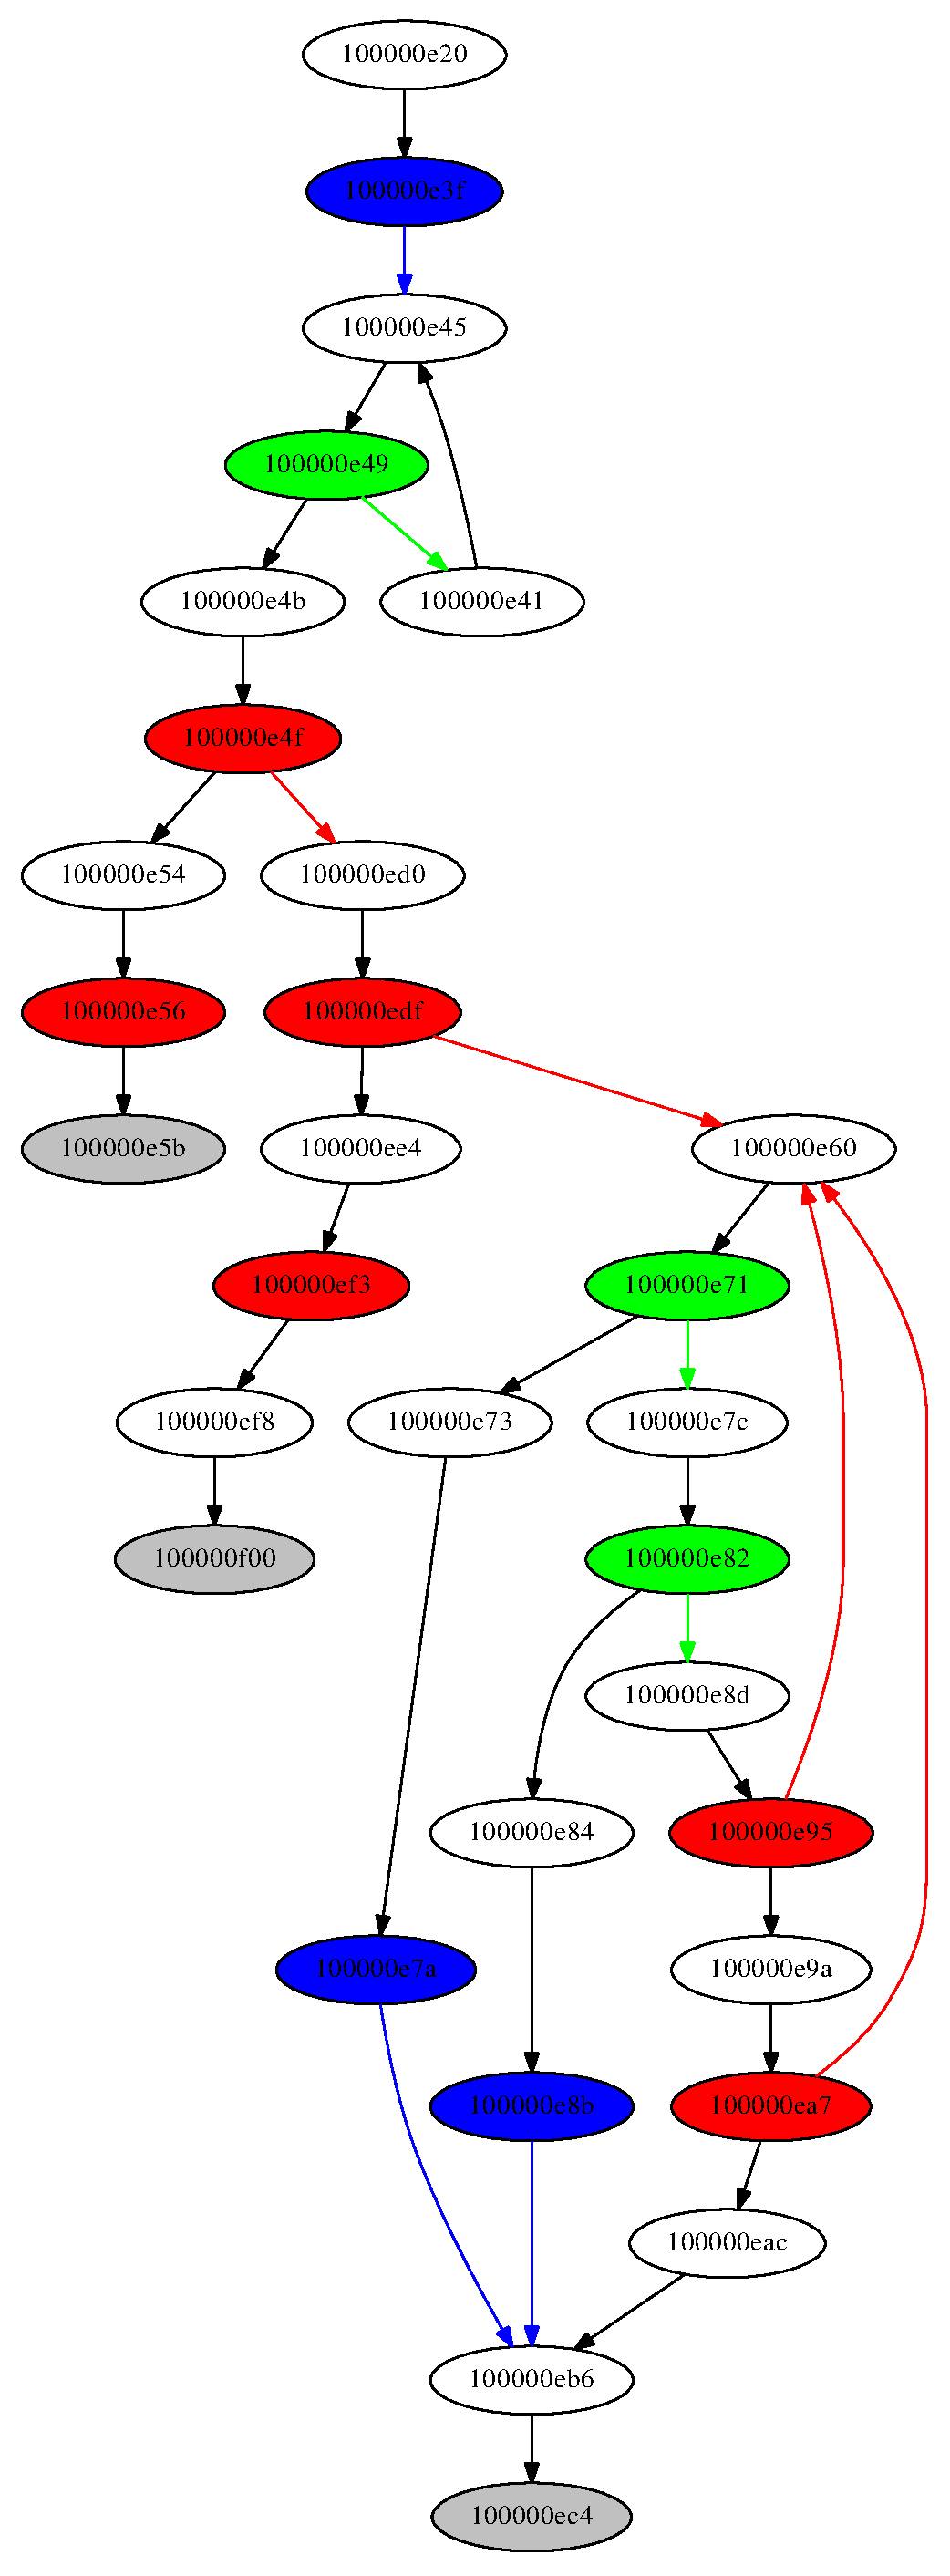
\includegraphics[width=7.4cm]{input/recc.eps}
%\caption{Graphe de flow de \texttt{fibo}}
%\label{CFGfibo}
%\end{figure}



\bibliographystyle{plain} 
\bibliography{biblio.bib}




%\section*{Conclusion}\input{input/ccl.tex}


\end{document}
	